% Options for packages loaded elsewhere
\PassOptionsToPackage{unicode}{hyperref}
\PassOptionsToPackage{hyphens}{url}
%
\documentclass[
]{article}
\usepackage{amsmath,amssymb}
\usepackage{lmodern}
\usepackage{iftex}
\ifPDFTeX
  \usepackage[T1]{fontenc}
  \usepackage[utf8]{inputenc}
  \usepackage{textcomp} % provide euro and other symbols
\else % if luatex or xetex
  \usepackage{unicode-math}
  \defaultfontfeatures{Scale=MatchLowercase}
  \defaultfontfeatures[\rmfamily]{Ligatures=TeX,Scale=1}
  \setmainfont[]{NEXON Lv2 Gothic}
\fi
% Use upquote if available, for straight quotes in verbatim environments
\IfFileExists{upquote.sty}{\usepackage{upquote}}{}
\IfFileExists{microtype.sty}{% use microtype if available
  \usepackage[]{microtype}
  \UseMicrotypeSet[protrusion]{basicmath} % disable protrusion for tt fonts
}{}
\makeatletter
\@ifundefined{KOMAClassName}{% if non-KOMA class
  \IfFileExists{parskip.sty}{%
    \usepackage{parskip}
  }{% else
    \setlength{\parindent}{0pt}
    \setlength{\parskip}{6pt plus 2pt minus 1pt}}
}{% if KOMA class
  \KOMAoptions{parskip=half}}
\makeatother
\usepackage{xcolor}
\usepackage[margin=1in]{geometry}
\usepackage{color}
\usepackage{fancyvrb}
\newcommand{\VerbBar}{|}
\newcommand{\VERB}{\Verb[commandchars=\\\{\}]}
\DefineVerbatimEnvironment{Highlighting}{Verbatim}{commandchars=\\\{\}}
% Add ',fontsize=\small' for more characters per line
\usepackage{framed}
\definecolor{shadecolor}{RGB}{248,248,248}
\newenvironment{Shaded}{\begin{snugshade}}{\end{snugshade}}
\newcommand{\AlertTok}[1]{\textcolor[rgb]{0.94,0.16,0.16}{#1}}
\newcommand{\AnnotationTok}[1]{\textcolor[rgb]{0.56,0.35,0.01}{\textbf{\textit{#1}}}}
\newcommand{\AttributeTok}[1]{\textcolor[rgb]{0.77,0.63,0.00}{#1}}
\newcommand{\BaseNTok}[1]{\textcolor[rgb]{0.00,0.00,0.81}{#1}}
\newcommand{\BuiltInTok}[1]{#1}
\newcommand{\CharTok}[1]{\textcolor[rgb]{0.31,0.60,0.02}{#1}}
\newcommand{\CommentTok}[1]{\textcolor[rgb]{0.56,0.35,0.01}{\textit{#1}}}
\newcommand{\CommentVarTok}[1]{\textcolor[rgb]{0.56,0.35,0.01}{\textbf{\textit{#1}}}}
\newcommand{\ConstantTok}[1]{\textcolor[rgb]{0.00,0.00,0.00}{#1}}
\newcommand{\ControlFlowTok}[1]{\textcolor[rgb]{0.13,0.29,0.53}{\textbf{#1}}}
\newcommand{\DataTypeTok}[1]{\textcolor[rgb]{0.13,0.29,0.53}{#1}}
\newcommand{\DecValTok}[1]{\textcolor[rgb]{0.00,0.00,0.81}{#1}}
\newcommand{\DocumentationTok}[1]{\textcolor[rgb]{0.56,0.35,0.01}{\textbf{\textit{#1}}}}
\newcommand{\ErrorTok}[1]{\textcolor[rgb]{0.64,0.00,0.00}{\textbf{#1}}}
\newcommand{\ExtensionTok}[1]{#1}
\newcommand{\FloatTok}[1]{\textcolor[rgb]{0.00,0.00,0.81}{#1}}
\newcommand{\FunctionTok}[1]{\textcolor[rgb]{0.00,0.00,0.00}{#1}}
\newcommand{\ImportTok}[1]{#1}
\newcommand{\InformationTok}[1]{\textcolor[rgb]{0.56,0.35,0.01}{\textbf{\textit{#1}}}}
\newcommand{\KeywordTok}[1]{\textcolor[rgb]{0.13,0.29,0.53}{\textbf{#1}}}
\newcommand{\NormalTok}[1]{#1}
\newcommand{\OperatorTok}[1]{\textcolor[rgb]{0.81,0.36,0.00}{\textbf{#1}}}
\newcommand{\OtherTok}[1]{\textcolor[rgb]{0.56,0.35,0.01}{#1}}
\newcommand{\PreprocessorTok}[1]{\textcolor[rgb]{0.56,0.35,0.01}{\textit{#1}}}
\newcommand{\RegionMarkerTok}[1]{#1}
\newcommand{\SpecialCharTok}[1]{\textcolor[rgb]{0.00,0.00,0.00}{#1}}
\newcommand{\SpecialStringTok}[1]{\textcolor[rgb]{0.31,0.60,0.02}{#1}}
\newcommand{\StringTok}[1]{\textcolor[rgb]{0.31,0.60,0.02}{#1}}
\newcommand{\VariableTok}[1]{\textcolor[rgb]{0.00,0.00,0.00}{#1}}
\newcommand{\VerbatimStringTok}[1]{\textcolor[rgb]{0.31,0.60,0.02}{#1}}
\newcommand{\WarningTok}[1]{\textcolor[rgb]{0.56,0.35,0.01}{\textbf{\textit{#1}}}}
\usepackage{longtable,booktabs,array}
\usepackage{calc} % for calculating minipage widths
% Correct order of tables after \paragraph or \subparagraph
\usepackage{etoolbox}
\makeatletter
\patchcmd\longtable{\par}{\if@noskipsec\mbox{}\fi\par}{}{}
\makeatother
% Allow footnotes in longtable head/foot
\IfFileExists{footnotehyper.sty}{\usepackage{footnotehyper}}{\usepackage{footnote}}
\makesavenoteenv{longtable}
\usepackage{graphicx}
\makeatletter
\def\maxwidth{\ifdim\Gin@nat@width>\linewidth\linewidth\else\Gin@nat@width\fi}
\def\maxheight{\ifdim\Gin@nat@height>\textheight\textheight\else\Gin@nat@height\fi}
\makeatother
% Scale images if necessary, so that they will not overflow the page
% margins by default, and it is still possible to overwrite the defaults
% using explicit options in \includegraphics[width, height, ...]{}
\setkeys{Gin}{width=\maxwidth,height=\maxheight,keepaspectratio}
% Set default figure placement to htbp
\makeatletter
\def\fps@figure{htbp}
\makeatother
\setlength{\emergencystretch}{3em} % prevent overfull lines
\providecommand{\tightlist}{%
  \setlength{\itemsep}{0pt}\setlength{\parskip}{0pt}}
\setcounter{secnumdepth}{-\maxdimen} % remove section numbering
\usepackage{booktabs}
\usepackage{longtable}
\usepackage{array}
\usepackage{multirow}
\usepackage{wrapfig}
\usepackage{float}
\usepackage{colortbl}
\usepackage{pdflscape}
\usepackage{tabu}
\usepackage{threeparttable}
\usepackage{threeparttablex}
\usepackage[normalem]{ulem}
\usepackage{makecell}
\usepackage{xcolor}
\ifLuaTeX
  \usepackage{selnolig}  % disable illegal ligatures
\fi
\IfFileExists{bookmark.sty}{\usepackage{bookmark}}{\usepackage{hyperref}}
\IfFileExists{xurl.sty}{\usepackage{xurl}}{} % add URL line breaks if available
\urlstyle{same} % disable monospaced font for URLs
\hypersetup{
  pdftitle={`메이플스토리' 관련 데이터 분석},
  pdfauthor={3504 김도윤},
  hidelinks,
  pdfcreator={LaTeX via pandoc}}

\title{`메이플스토리' 관련 데이터 분석}
\author{3504 김도윤}
\date{2022-09-13}

\begin{document}
\maketitle

\hypertarget{uxc11cuxbb38}{%
\section{서문}\label{uxc11cuxbb38}}

'메이플스토리'는 2003년부터 서비스되기 시작한 온라인 MMORPG 게임으로, 꽤
많은 유저들이 지금까지도 즐기고 있다.

이 게임는 캐릭터를 자신이 만들고 45개의 직업 중 1개를 선택하여 스토리 및
관련 컨텐츠를 즐기는 게임으로, 다양한 사용자들이 12개의 서버 중 1개의
서버를 주로 선택한 후 컨텐츠를 즐긴다.

서버 당 캐릭터의 생성 제한 수도 정해져있고, 모든 캐릭터에 시간을
동등하게 쓸 수 있는 건 아니기에 대부분의 사람들은 '주캐릭터'를 한 개
정하여 그 캐릭터들에게 장비 및 경험치를 몰아주는 편이다.

최근에는 (22년 8월) 여름 업데이트로 신규 맵 및 밸런스 패치가 진행되면서
관련 커뮤니티에서는 어떠한 직업이 상향을 받았는지 혹은 받지 않았는지,
변경점은 무엇인지 파악하면서 직업 간 비교를 하였다.

대체로 상향을 받았지만, 어떤 직업들은 상향을 받지 못했음에도 불구하고
해당 직업을 '주캐릭터'로 하는 사람이 적어 알아주는 사람이 적다고
하소연하는 상황도 있었다.

이에 이러한 직업간 편차가 실제로 존재하는지 알아보기 위해서 본 분석을
진행해보았다.

\hypertarget{uxcd94uxcd9c-uxbc29uxbc95}{%
\section{추출 방법}\label{uxcd94uxcd9c-uxbc29uxbc95}}

분석을 해보기 전에, 관련 데이터를 가져와야 한다. 이는 Maple.gg 사이트의
`통합 랭킹' 부분에서 파싱해왔다. 파싱 날짜는 2022년 8월 17일 오후 6시
50분 경이다.

추출한 데이터는 다음과 같다 :

\begin{itemize}
\item
  `통합 랭킹' 페이지의 `일반 랭킹'의 '전체' 항목의 1위부터 50000위까지의
  닉네임, 레벨, 직업, 인기도, 길드 데이터.
\item
  `통합 랭킹' 페이지의 '일반 랭킹'의 각 서버(12개)\footnote{루나,
    스카니아, 엘리시움, 크로아, 오로라, 베라, 레드, 유니온, 제니스,
    이노시스, 아케인, 노바} \footnote{리부트 서버(1, 2)는 포함하지
    않았음}의 1위부터 10000위까지의 닉네임, 레벨, 직업, 인기도, 길드
  데이터.
\end{itemize}

데이터를 가져온 파일의 소스코드는 다음과 같다. 이는 Python으로
작성되었다.

\begin{itemize}
\tightlist
\item
  `전체' 항목 가져오기
\end{itemize}

\begin{Shaded}
\begin{Highlighting}[]
\ImportTok{import}\NormalTok{ requests}
\ImportTok{from}\NormalTok{ bs4 }\ImportTok{import}\NormalTok{ BeautifulSoup}

\CommentTok{\# 전체 랭킹 1\textasciitilde{}50000위}
\NormalTok{list1 }\OperatorTok{=} \BuiltInTok{list}\NormalTok{()}

\ControlFlowTok{for}\NormalTok{ i }\KeywordTok{in} \BuiltInTok{range}\NormalTok{(}\DecValTok{1}\NormalTok{, }\DecValTok{2501}\NormalTok{, }\DecValTok{1}\NormalTok{) :}
\NormalTok{    url }\OperatorTok{=} \StringTok{\textquotesingle{}https://maple.gg/rank/total?page=}\SpecialCharTok{\%s}\StringTok{\textquotesingle{}}\OperatorTok{\%}\NormalTok{ i}
\NormalTok{    response }\OperatorTok{=}\NormalTok{ requests.get(url)}
    \BuiltInTok{print}\NormalTok{(}\BuiltInTok{str}\NormalTok{(i), response.status\_code)}
\NormalTok{    html }\OperatorTok{=}\NormalTok{ response.text}
\NormalTok{    soup }\OperatorTok{=}\NormalTok{ BeautifulSoup(html, }\StringTok{\textquotesingle{}html.parser\textquotesingle{}}\NormalTok{)}
    \ControlFlowTok{for}\NormalTok{ j }\KeywordTok{in} \BuiltInTok{range}\NormalTok{(}\DecValTok{1}\NormalTok{,}\DecValTok{21}\NormalTok{,}\DecValTok{1}\NormalTok{) :}
\NormalTok{        nickname }\OperatorTok{=}\NormalTok{ soup.select\_one(}\StringTok{\textquotesingle{}.table \textgreater{} tbody:nth{-}child(3) \textgreater{} tr:nth{-}child(}\SpecialCharTok{\%s}\StringTok{) \textgreater{} td:nth{-}child(2) \textgreater{} div:nth{-}child(2) \textgreater{} span:nth{-}child(2) \textgreater{} a:nth{-}child(1)\textquotesingle{}}\OperatorTok{\%}\NormalTok{j).text}
\NormalTok{        level }\OperatorTok{=}\NormalTok{ soup.select\_one(}\StringTok{\textquotesingle{}.table \textgreater{} tbody:nth{-}child(3) \textgreater{} tr:nth{-}child(}\SpecialCharTok{\%s}\StringTok{) \textgreater{} td:nth{-}child(2) \textgreater{} div:nth{-}child(2) \textgreater{} div:nth{-}child(3) \textgreater{} span:nth{-}child(1)\textquotesingle{}}\OperatorTok{\%}\NormalTok{j).text}
\NormalTok{        job }\OperatorTok{=}\NormalTok{ soup.select\_one(}\StringTok{\textquotesingle{}.table \textgreater{} tbody:nth{-}child(3) \textgreater{} tr:nth{-}child(}\SpecialCharTok{\%s}\StringTok{) \textgreater{} td:nth{-}child(2) \textgreater{} div:nth{-}child(2) \textgreater{} div:nth{-}child(3) \textgreater{} span:nth{-}child(4)\textquotesingle{}}\OperatorTok{\%}\NormalTok{j).text}
\NormalTok{        inki }\OperatorTok{=}\NormalTok{ soup.select\_one(}\StringTok{\textquotesingle{}.table \textgreater{} tbody:nth{-}child(3) \textgreater{} tr:nth{-}child(}\SpecialCharTok{\%s}\StringTok{) \textgreater{} td:nth{-}child(3)\textquotesingle{}}\OperatorTok{\%}\NormalTok{j).text}
        \ControlFlowTok{try}\NormalTok{ :}
\NormalTok{            guild }\OperatorTok{=}\NormalTok{ soup.select\_one(}\StringTok{\textquotesingle{}.table \textgreater{} tbody:nth{-}child(3) \textgreater{} tr:nth{-}child(}\SpecialCharTok{\%s}\StringTok{) \textgreater{} td:nth{-}child(4) \textgreater{} a:nth{-}child(1)\textquotesingle{}}\OperatorTok{\%}\NormalTok{j).text}
        \ControlFlowTok{except}\NormalTok{ :}
\NormalTok{            guild }\OperatorTok{=} \StringTok{\textquotesingle{}{-}{-} 없음 {-}{-}\textquotesingle{}}
\NormalTok{        string }\OperatorTok{=}\NormalTok{ nickname }\OperatorTok{+} \StringTok{\textquotesingle{},\textquotesingle{}} \OperatorTok{+}\NormalTok{ level }\OperatorTok{+} \StringTok{\textquotesingle{},\textquotesingle{}} \OperatorTok{+}\NormalTok{ job }\OperatorTok{+} \StringTok{\textquotesingle{},\textquotesingle{}} \OperatorTok{+}\NormalTok{ inki }\OperatorTok{+} \StringTok{\textquotesingle{},\textquotesingle{}} \OperatorTok{+}\NormalTok{ guild.replace(}\StringTok{\textquotesingle{} \textquotesingle{}}\NormalTok{,}\StringTok{\textquotesingle{}\textquotesingle{}}\NormalTok{).replace(}\StringTok{\textquotesingle{}}\CharTok{\textbackslash{}n}\StringTok{\textquotesingle{}}\NormalTok{,}\StringTok{\textquotesingle{}\textquotesingle{}}\NormalTok{)}
        \CommentTok{\#print(string)}
\NormalTok{        list1.append(string)}
    \CommentTok{\#print(list1, len(list1))}
\NormalTok{a }\OperatorTok{=} \BuiltInTok{open}\NormalTok{(}\StringTok{\textquotesingle{}ranking\_all.csv\textquotesingle{}}\NormalTok{, }\StringTok{\textquotesingle{}w\textquotesingle{}}\NormalTok{,encoding}\OperatorTok{=}\StringTok{\textquotesingle{}utf{-}8\textquotesingle{}}\NormalTok{)}
\ControlFlowTok{for}\NormalTok{ i }\KeywordTok{in} \BuiltInTok{range}\NormalTok{(}\DecValTok{0}\NormalTok{, }\BuiltInTok{len}\NormalTok{(list1), }\DecValTok{1}\NormalTok{) :}
\NormalTok{    a.write(list1[i] }\OperatorTok{+} \StringTok{\textquotesingle{}}\CharTok{\textbackslash{}n}\StringTok{\textquotesingle{}}\NormalTok{)}
\NormalTok{a.close()}
\end{Highlighting}
\end{Shaded}

\begin{itemize}
\tightlist
\item
  `각 서버별' 항목 가져오기
\end{itemize}

\begin{Shaded}
\begin{Highlighting}[]
\ImportTok{import}\NormalTok{ requests}
\ImportTok{from}\NormalTok{ bs4 }\ImportTok{import}\NormalTok{ BeautifulSoup}

\CommentTok{\# 서버 별 1\textasciitilde{}10000위}
\CommentTok{\#serverlist = [\textquotesingle{}luna\textquotesingle{}, \textquotesingle{}elysium\textquotesingle{}, \textquotesingle{}croa\textquotesingle{}, \textquotesingle{}aurora\textquotesingle{},\textquotesingle{}bera\textquotesingle{},\textquotesingle{}red\textquotesingle{},\textquotesingle{}union\textquotesingle{},\textquotesingle{}zenith\textquotesingle{},\textquotesingle{}enosis\textquotesingle{},\textquotesingle{}arcane\textquotesingle{},\textquotesingle{}nova\textquotesingle{}]}
\NormalTok{serverlist }\OperatorTok{=}\NormalTok{ [}\StringTok{\textquotesingle{}scania\textquotesingle{}}\NormalTok{]}
\ControlFlowTok{for}\NormalTok{ i }\KeywordTok{in}\NormalTok{ serverlist :}
\NormalTok{    list1 }\OperatorTok{=} \BuiltInTok{list}\NormalTok{()}
    \ControlFlowTok{for}\NormalTok{ j }\KeywordTok{in} \BuiltInTok{range}\NormalTok{(}\DecValTok{1}\NormalTok{, }\DecValTok{501}\NormalTok{, }\DecValTok{1}\NormalTok{) :}
\NormalTok{        url }\OperatorTok{=} \StringTok{\textquotesingle{}https://maple.gg/rank/total/}\SpecialCharTok{\%s}\StringTok{?page=}\SpecialCharTok{\%s}\StringTok{\textquotesingle{}}\OperatorTok{\%}\NormalTok{ (i, j)}
\NormalTok{        response }\OperatorTok{=}\NormalTok{ requests.get(url)}
        \BuiltInTok{print}\NormalTok{(}\BuiltInTok{str}\NormalTok{(i), }\BuiltInTok{str}\NormalTok{(j), response.status\_code)}
\NormalTok{        html }\OperatorTok{=}\NormalTok{ response.text}
\NormalTok{        soup }\OperatorTok{=}\NormalTok{ BeautifulSoup(html, }\StringTok{\textquotesingle{}html.parser\textquotesingle{}}\NormalTok{)}
        \ControlFlowTok{for}\NormalTok{ k }\KeywordTok{in} \BuiltInTok{range}\NormalTok{(}\DecValTok{1}\NormalTok{,}\DecValTok{21}\NormalTok{,}\DecValTok{1}\NormalTok{) :}
\NormalTok{            nickname }\OperatorTok{=}\NormalTok{ soup.select\_one(}\StringTok{\textquotesingle{}.table \textgreater{} tbody:nth{-}child(3) \textgreater{} tr:nth{-}child(}\SpecialCharTok{\%s}\StringTok{) \textgreater{} td:nth{-}child(2) \textgreater{} div:nth{-}child(2) \textgreater{} span:nth{-}child(2) \textgreater{} a:nth{-}child(1)\textquotesingle{}}\OperatorTok{\%}\NormalTok{k).text}
\NormalTok{            level }\OperatorTok{=}\NormalTok{ soup.select\_one(}\StringTok{\textquotesingle{}.table \textgreater{} tbody:nth{-}child(3) \textgreater{} tr:nth{-}child(}\SpecialCharTok{\%s}\StringTok{) \textgreater{} td:nth{-}child(2) \textgreater{} div:nth{-}child(2) \textgreater{} div:nth{-}child(3) \textgreater{} span:nth{-}child(1)\textquotesingle{}}\OperatorTok{\%}\NormalTok{k).text}
\NormalTok{            job }\OperatorTok{=}\NormalTok{ soup.select\_one(}\StringTok{\textquotesingle{}.table \textgreater{} tbody:nth{-}child(3) \textgreater{} tr:nth{-}child(}\SpecialCharTok{\%s}\StringTok{) \textgreater{} td:nth{-}child(2) \textgreater{} div:nth{-}child(2) \textgreater{} div:nth{-}child(3) \textgreater{} span:nth{-}child(4)\textquotesingle{}}\OperatorTok{\%}\NormalTok{k).text.replace(}\StringTok{\textquotesingle{},\textquotesingle{}}\NormalTok{,}\StringTok{\textquotesingle{}\textquotesingle{}}\NormalTok{)}
\NormalTok{            inki }\OperatorTok{=}\NormalTok{ soup.select\_one(}\StringTok{\textquotesingle{}.table \textgreater{} tbody:nth{-}child(3) \textgreater{} tr:nth{-}child(}\SpecialCharTok{\%s}\StringTok{) \textgreater{} td:nth{-}child(3)\textquotesingle{}}\OperatorTok{\%}\NormalTok{k).text.replace(}\StringTok{\textquotesingle{},\textquotesingle{}}\NormalTok{,}\StringTok{\textquotesingle{}\textquotesingle{}}\NormalTok{)}
            \ControlFlowTok{try}\NormalTok{ :}
\NormalTok{                guild }\OperatorTok{=}\NormalTok{ soup.select\_one(}\StringTok{\textquotesingle{}.table \textgreater{} tbody:nth{-}child(3) \textgreater{} tr:nth{-}child(}\SpecialCharTok{\%s}\StringTok{) \textgreater{} td:nth{-}child(4) \textgreater{} a:nth{-}child(1)\textquotesingle{}}\OperatorTok{\%}\NormalTok{k).text}
            \ControlFlowTok{except}\NormalTok{ :}
\NormalTok{                guild }\OperatorTok{=} \StringTok{\textquotesingle{}{-}{-} 없음 {-}{-}\textquotesingle{}}
\NormalTok{            string }\OperatorTok{=}\NormalTok{ nickname }\OperatorTok{+} \StringTok{\textquotesingle{},\textquotesingle{}} \OperatorTok{+}\NormalTok{ level }\OperatorTok{+} \StringTok{\textquotesingle{},\textquotesingle{}} \OperatorTok{+}\NormalTok{ job }\OperatorTok{+} \StringTok{\textquotesingle{},\textquotesingle{}} \OperatorTok{+}\NormalTok{ inki }\OperatorTok{+} \StringTok{\textquotesingle{},\textquotesingle{}} \OperatorTok{+}\NormalTok{ guild.replace(}\StringTok{\textquotesingle{} \textquotesingle{}}\NormalTok{,}\StringTok{\textquotesingle{}\textquotesingle{}}\NormalTok{).replace(}\StringTok{\textquotesingle{}}\CharTok{\textbackslash{}n}\StringTok{\textquotesingle{}}\NormalTok{,}\StringTok{\textquotesingle{}\textquotesingle{}}\NormalTok{)}
            \CommentTok{\#print(string)}
\NormalTok{            list1.append(string)}
        \CommentTok{\#print(list1, len(list1))}
\NormalTok{    a }\OperatorTok{=} \BuiltInTok{open}\NormalTok{(}\StringTok{\textquotesingle{}ranking\_}\SpecialCharTok{\%s}\StringTok{.csv\textquotesingle{}}\OperatorTok{\%}\NormalTok{ i, }\StringTok{\textquotesingle{}w\textquotesingle{}}\NormalTok{,encoding}\OperatorTok{=}\StringTok{\textquotesingle{}utf{-}8\textquotesingle{}}\NormalTok{)}
    \ControlFlowTok{for}\NormalTok{ i }\KeywordTok{in} \BuiltInTok{range}\NormalTok{(}\DecValTok{0}\NormalTok{, }\BuiltInTok{len}\NormalTok{(list1), }\DecValTok{1}\NormalTok{) :}
\NormalTok{        a.write(list1[i] }\OperatorTok{+} \StringTok{\textquotesingle{}}\CharTok{\textbackslash{}n}\StringTok{\textquotesingle{}}\NormalTok{)}
\NormalTok{    a.close()}
\end{Highlighting}
\end{Shaded}

위 데이터의 명칭을 지금부터 `전체 랭킹', '서버 랭킹'으로 갈음한다.

\hypertarget{uxb370uxc774uxd130-uxbd84uxc11d}{%
\section{데이터 분석}\label{uxb370uxc774uxd130-uxbd84uxc11d}}

\hypertarget{uxc804uxccb4-uxb7aduxd0b9}{%
\subsection{전체 랭킹}\label{uxc804uxccb4-uxb7aduxd0b9}}

\hypertarget{uxc9c1uxc5c5uxacfc-uxb808uxbca8}{%
\subsubsection{직업과 레벨}\label{uxc9c1uxc5c5uxacfc-uxb808uxbca8}}

\hypertarget{uxc804uxccb4-uxc9c1uxc5c5-uxbd84uxd3ec}{%
\paragraph{전체 직업
분포}\label{uxc804uxccb4-uxc9c1uxc5c5-uxbd84uxd3ec}}

직업간 편차를 알기 위해 가장 먼저 해본 것은 `전체 랭킹'에서의 직업의
비율을 알아보는 것이다. 특정 직업이 더 많은 비율을 실제로 차지하고
있는지, 있다면 어느 직업인지를 알아보기 위해서이다. 따라서 '전체
랭킹'에서 '직업' 항목만 따로 떼어서 각 빈도 수를 체크하여 보았다.

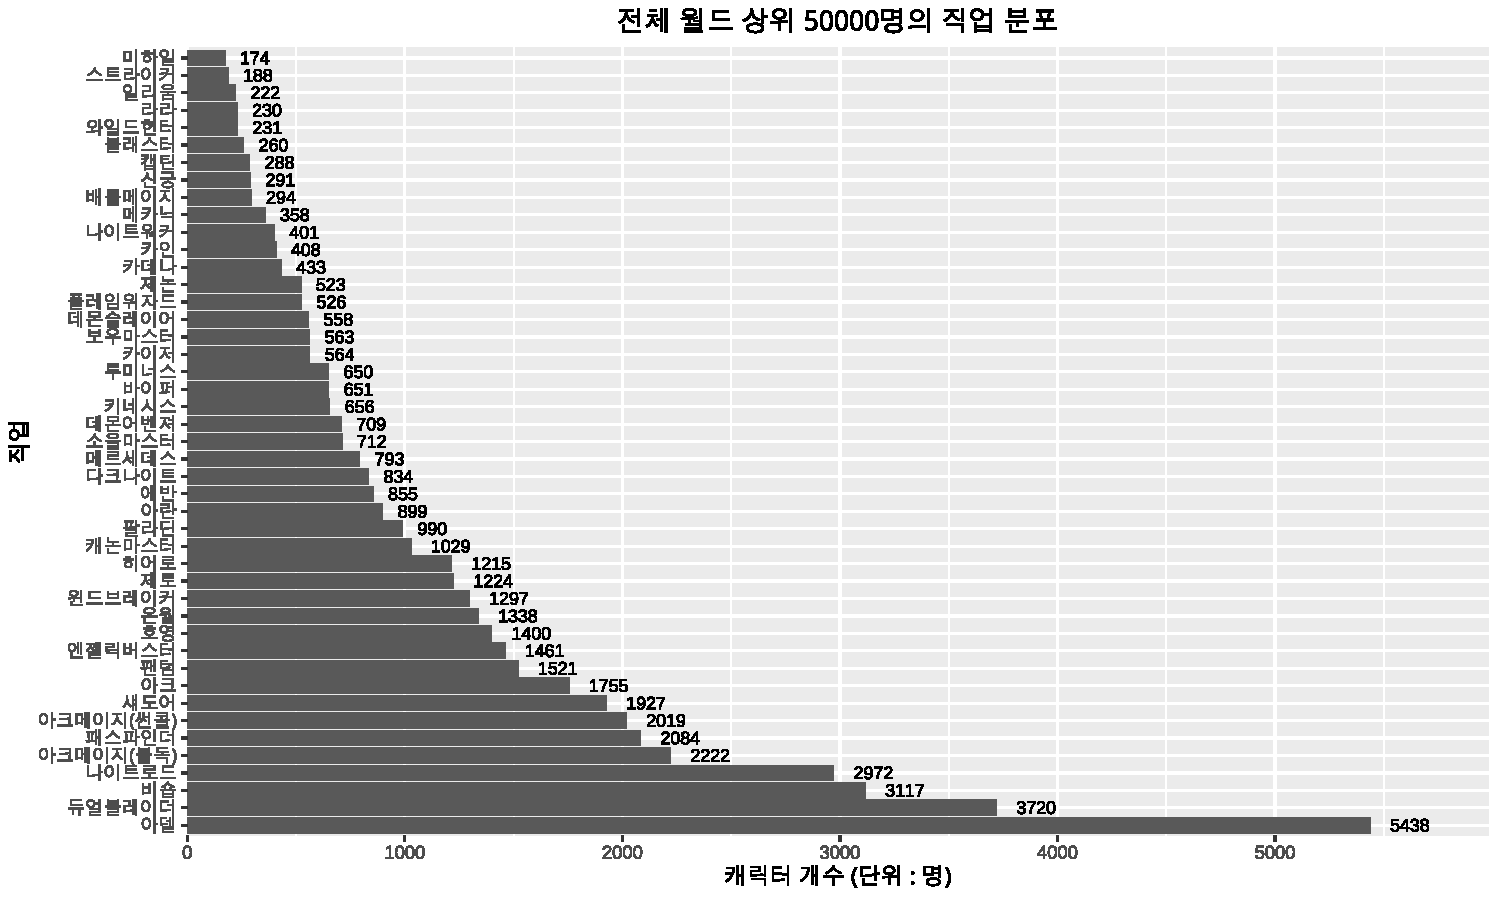
\includegraphics{123_files/figure-latex/ranking_all_job-1.pdf}

\begin{table}[H]

\centering
\begin{tabular}[t]{lr}
\toprule
직업 & 비율\\
\midrule
아델 & 10.88\\
듀얼블레이더 & 7.44\\
비숍 & 6.23\\
나이트로드 & 5.94\\
아크메이지(불독) & 4.44\\
\addlinespace
패스파인더 & 4.17\\
아크메이지(썬콜) & 4.04\\
섀도어 & 3.85\\
아크 & 3.51\\
팬텀 & 3.04\\
\addlinespace
엔젤릭버스터 & 2.92\\
호영 & 2.80\\
은월 & 2.68\\
윈드브레이커 & 2.59\\
제로 & 2.45\\
\bottomrule
\end{tabular}
\centering
\begin{tabular}[t]{lr}
\toprule
직업 & 비율\\
\midrule
히어로 & 2.43\\
캐논마스터 & 2.06\\
팔라딘 & 1.98\\
아란 & 1.80\\
에반 & 1.71\\
\addlinespace
다크나이트 & 1.67\\
메르세데스 & 1.59\\
데몬어벤져 & 1.42\\
소울마스터 & 1.42\\
키네시스 & 1.31\\
\addlinespace
루미너스 & 1.30\\
바이퍼 & 1.30\\
보우마스터 & 1.13\\
카이저 & 1.13\\
데몬슬레이어 & 1.12\\
\bottomrule
\end{tabular}
\centering
\begin{tabular}[t]{lr}
\toprule
직업 & 비율\\
\midrule
제논 & 1.05\\
플레임위자드 & 1.05\\
카데나 & 0.87\\
카인 & 0.82\\
나이트워커 & 0.80\\
\addlinespace
메카닉 & 0.72\\
배틀메이지 & 0.59\\
신궁 & 0.58\\
캡틴 & 0.58\\
블래스터 & 0.52\\
\addlinespace
라라 & 0.46\\
와일드헌터 & 0.46\\
일리움 & 0.44\\
스트라이커 & 0.38\\
미하일 & 0.35\\
\bottomrule
\end{tabular}
\end{table}

비율의 단위는 퍼센트(\%)이며, 소숫점 2자리에서 반올림하였다.

`아델(5438명, 10.88\%)'이 혼자 두자리수 점유율을 가져가며 2위인
'듀얼블레이더(3720명, 7.44\%)'를 큰 차이로 앞서고 있으며, '비숍(3117명,
6.23\%)', `나이트로드(2972명, 5.94\%')이 뒤를 잇고 있다. 가장 적은
랭커를 가진 직업은 '미하일(174명, 0.35\%)'이었다. '미하일'과 '아델'은 약
31배 차이가 난다.

메이플스토리 관련 커뮤니티에서는 타 직업 대비 효율 등이 좋은 직업들(속칭
`(0)1티어' 직업들)을 엮어 부르는 경향이 있다. 이와 관련 데이터를
비교해보면 다음과 같다 :

\begin{itemize}
\item
  `호아아' (호영(12위), 아델(\textbf{\textcolor{blue}{1위}}), 아크(9위))
  - 가장 오랫동안 언급되었던 직업인 만큼 상위권에 위치해있다.
\item
  `나로호독' (나이트로드 (\textbf{4위}), 호영(12위),
  아크메이지(불독)(\textbf{5위})) - 모험가 리마스터(22년 1월 경)부터
  후술할 '데은불닼'이 나오기 전까지 언급되었던 직업들. 역시 상위권에
  위치해있다.
\item
  `데은불닼'(`은데불닼') (데몬어벤져 (\textbf{\textcolor{red}{23위}}),
  은월(13위), 아크메이지(불독)(\textbf{5위}), 다크나이트(21위)) 2022년
  4월 밸런스패치 이후로 언급되었던 직업들. 현재 (2022년 8월 기준)도
  언급되고 있다. 패치와 리마스터로 좋아진 직업들이 많기에 시간을 많이
  투자해야 하는 상위권에는 아직 분포가 적은 모습을 볼 수 있다.
\end{itemize}

\hypertarget{uxb808uxbca8uxbcc4-uxc9c1uxc5c5-uxbd84uxd3ec}{%
\paragraph{레벨별 직업
분포}\label{uxb808uxbca8uxbcc4-uxc9c1uxc5c5-uxbd84uxd3ec}}

'메이플스토리'는 레벨이라는 시스템이 존재한다. 레벨에 따라 스토리가
해금되고 캐릭터의 능력치가 좋아지는 등의 전형적인 RPG 시스템이다. 최고
레벨은 300레벨이며, 1레벨 부터 9레벨은 0차 전직, 10레벨부터 29레벨은 1차
전직, 30레벨부터 59레벨은 2차 전직, 60레벨부터 99레벨까지는 3차 전직,
100레벨부터 200레벨까지는 4차 전직으로 분류된다. 200레벨 이상은 5차
전직으로 분류되는데, 이 5차 전직부터 메이플스토리의 대부분 기능이
해금되기에 대부분의 주력 캐릭터는 5차 전직을 완료한 상태이다.

또한 1레벨부터 200레벨까지의 레벨을 올리는 것은 쉬우나, 200레벨부턴
레벨업을 하는데 어려움이 따른다.

따라서 레벨은 단순히 강함을 표시하는 수치도 되지만, 얼마나 오랫동안
캐릭터를 육성해왔는지에 대한 의미도 내포하는 수치도 된다는 것이다.

그렇다면 이 직업들의 레벨 간에도 차이가 있을까? 이를 알아보기 위해서 각
레벨에 어느 직업이 분포되어있는지를 파악해보기로 하였다.

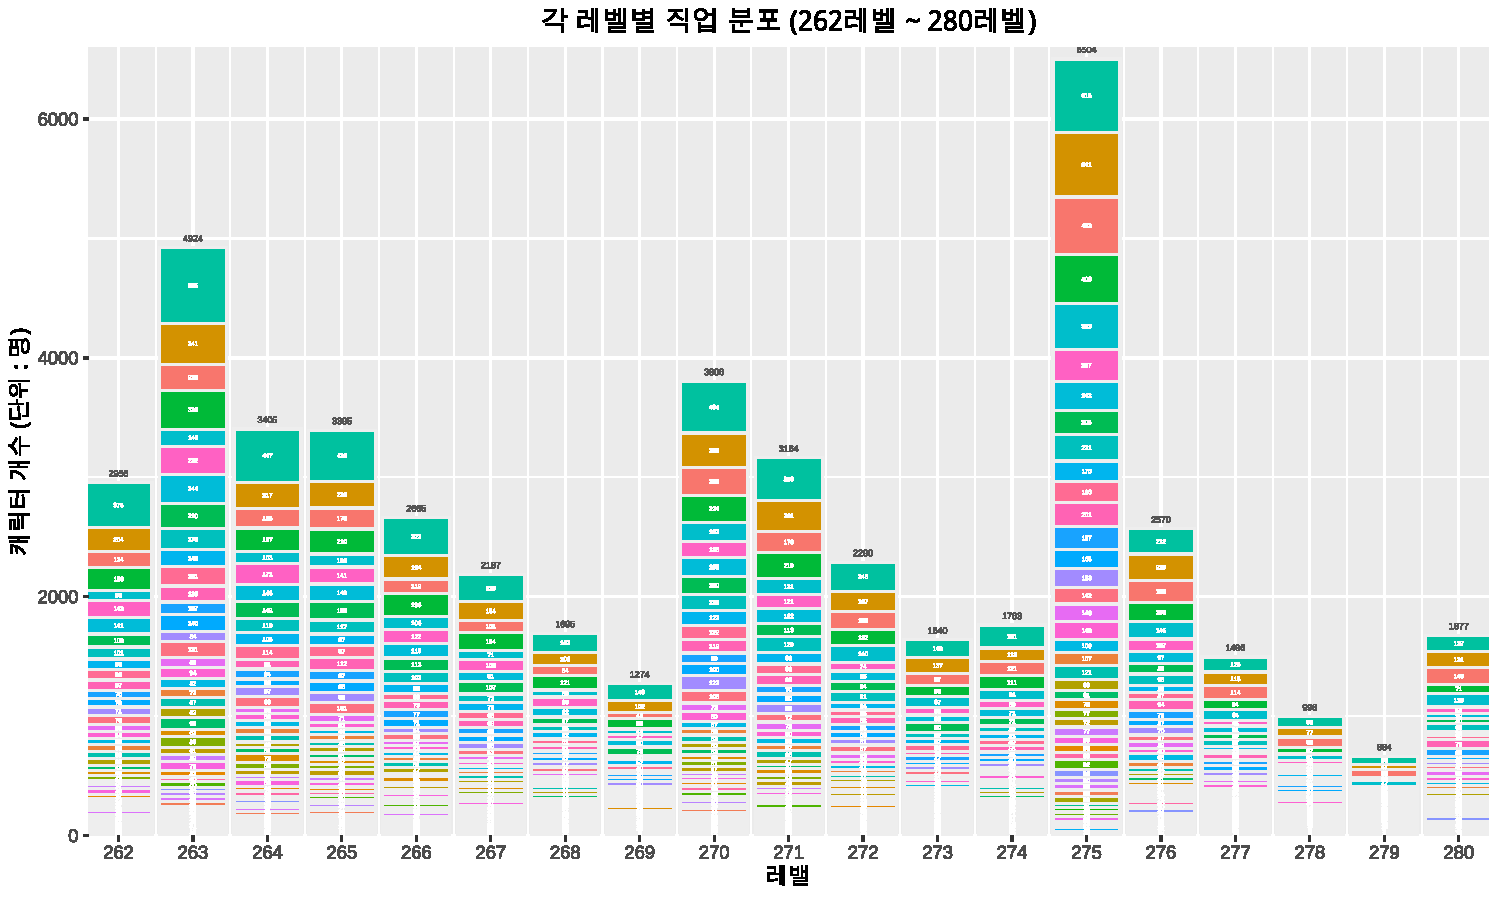
\includegraphics{123_files/figure-latex/ranking_all_level_job-1.pdf}
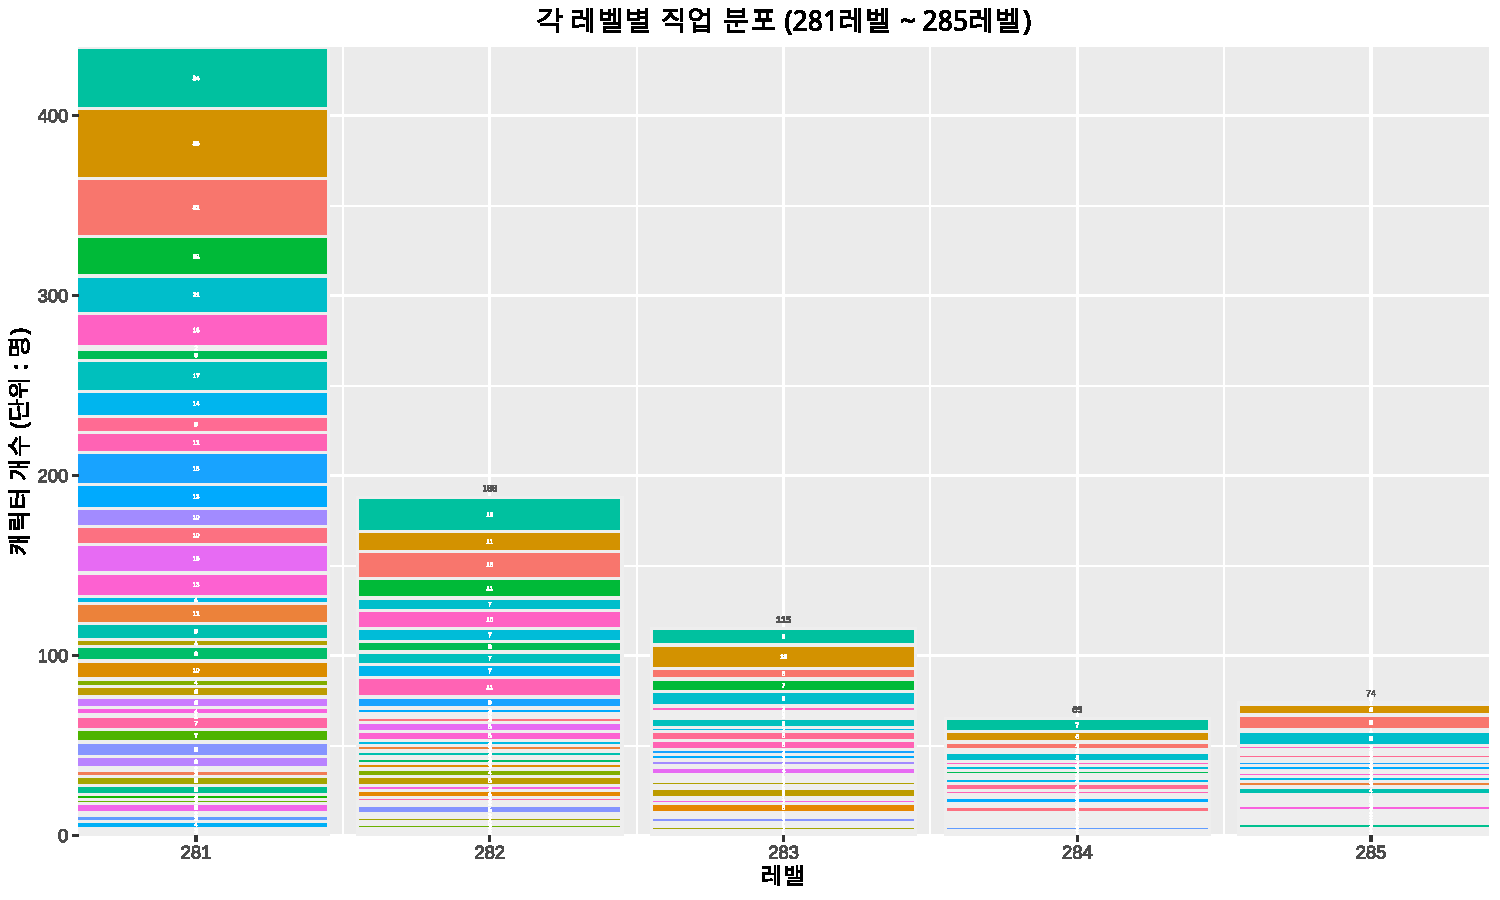
\includegraphics{123_files/figure-latex/ranking_all_level_job-2.pdf}
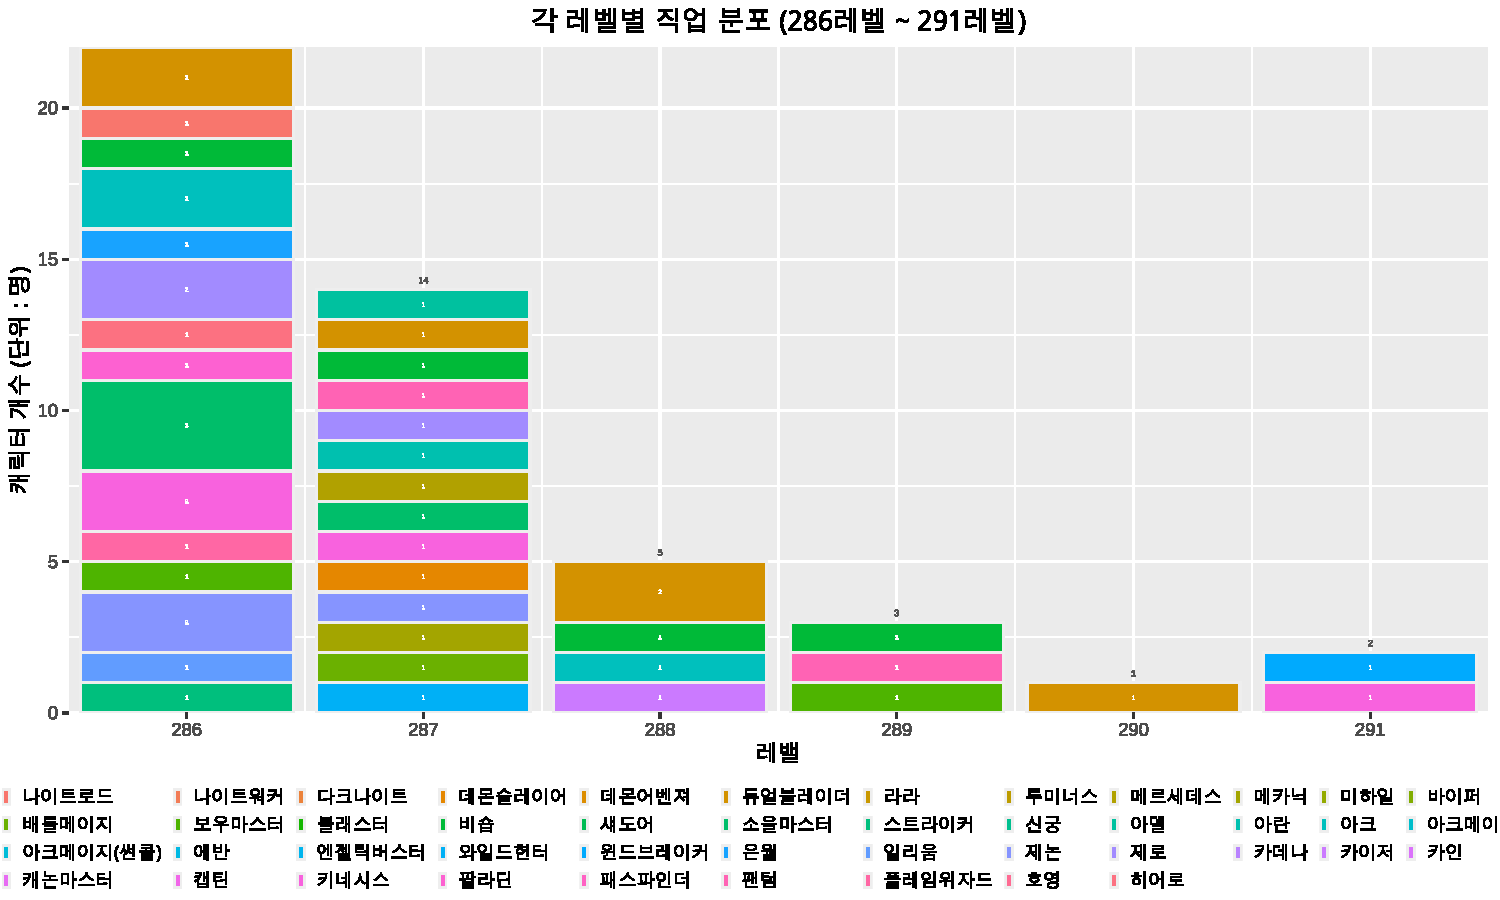
\includegraphics{123_files/figure-latex/ranking_all_level_job-3.pdf}

\begin{table}[H]

\centering
\begin{tabular}[t]{lr}
\toprule
레밸 & 전체인원\\
\midrule
262 & 2956\\
263 & 4924\\
264 & 3405\\
265 & 3395\\
266 & 2665\\
\addlinespace
267 & 2187\\
268 & 1695\\
269 & 1274\\
270 & 3806\\
271 & 3164\\
\bottomrule
\end{tabular}
\centering
\begin{tabular}[t]{lr}
\toprule
레밸 & 전체인원\\
\midrule
272 & 2290\\
273 & 1640\\
274 & 1763\\
275 & 6504\\
276 & 2570\\
\addlinespace
277 & 1496\\
278 & 998\\
279 & 664\\
280 & 1677\\
281 & 438\\
\bottomrule
\end{tabular}
\centering
\begin{tabular}[t]{lr}
\toprule
레밸 & 전체인원\\
\midrule
282 & 188\\
283 & 115\\
284 & 65\\
285 & 74\\
286 & 22\\
\addlinespace
287 & 14\\
288 & 5\\
289 & 3\\
290 & 1\\
291 & 2\\
\bottomrule
\end{tabular}
\end{table}

가장 많은 캐릭터를 가지고 있는 분류는 263레벨의 아델(635명) 이다. 그
뒤는 275레벨의 아델(615명), 275레벨의 듀얼블레이더(541명)이다.

또한 대부분의 많은 캐릭터가 275레벨(6504명)과 263레벨(4924명),
270레벨(3806명)에 머물러 있다는 것을 알 수 있다.

281레벨부터 285레벨까지는 대체로 100명에서 500명 사이의 캐릭터만이
있었으며, 286레벨부터는 1명에서 20명 사이의 캐릭터만이 있었다. 최고
레벨은 291레벨이었다.\footnote{게임 최고 레벨은 300레벨.}

각 직업별 최고 레벨과 각 직업별 최다 분포의 레벨은 다음과 같다.
평균레벨은 소숫점 2자리에서 반올림하였다. 정렬은 평균레벨 순이다.

\begin{longtable}[]{@{}
  >{\raggedright\arraybackslash}p{(\columnwidth - 6\tabcolsep) * \real{0.1333}}
  >{\raggedright\arraybackslash}p{(\columnwidth - 6\tabcolsep) * \real{0.2593}}
  >{\raggedright\arraybackslash}p{(\columnwidth - 6\tabcolsep) * \real{0.3259}}
  >{\raggedright\arraybackslash}p{(\columnwidth - 6\tabcolsep) * \real{0.2815}}@{}}
\toprule()
\begin{minipage}[b]{\linewidth}\raggedright
직업
\end{minipage} & \begin{minipage}[b]{\linewidth}\raggedright
최고레벨
\end{minipage} & \begin{minipage}[b]{\linewidth}\raggedright
최다레벨(인원수)
\end{minipage} & \begin{minipage}[b]{\linewidth}\raggedright
평균레벨
\end{minipage} \\
\midrule()
\endhead
와일드헌터 & 287 & 275(35) & \textbf{\textcolor{blue}{271.57}} \\
아크메이지(불독) & 285 & 275(383) & 271.55 \\
제논 & 287 & 275(66) & 271.53 \\
나이트로드 & 286 & 275(483) & 271.23 \\
메카닉 & 287 & 275(59) & 270.96 \\
캐논마스터 & 283 & 275(148) & 270.76 \\
은월 & 286 & 275(187) & 270.72 \\
팔라딘 & 286 & 275(148) & 270.72 \\
캡틴 & 285 & 275(46) & 270.64 \\
팬텀 & 289 & 275(201) & 270.58 \\
보우마스터 & 289 & 275(82) & 270.54 \\
플레임위자드 & 286 & 275(63) & 270.53 \\
듀얼블레이더 & 290 & 275(541) & 270.44 \\
일리움 & 286 & 275(22) & 270.36 \\
배틀메이지 & 287 & 275(38) & 270.32 \\
아란 & 287 & 275(121) & 270.27 \\
제로 & 287 & 275(153) & 270.27 \\
데몬슬레이어 & 287 & 275(66) & 270.25 \\
에반 & 285 & 275(109) & 270.25 \\
블래스터 & \textbf{\textcolor{red}{281}} & 275(35) & 270.17 \\
윈드브레이커 & \textbf{\textcolor{blue}{291}} & 275(165) & 270.15 \\
루미너스 & 285 & 275(72) & 270.11 \\
\textbf{전체} & \textbf{291} & \textbf{275(6504)} & \textbf{270.06} \\
아크 & 288 & 275(221) & 270.04 \\
카데나 & 285 & 275(50) & 270.03 \\
메르세데스 & 287 & 275(88) & 269.95 \\
다크나이트 & 285 & 275(107) & 269.97 \\
스트라이커 & 286 & \textcolor{red}{263(25)} & 269.82 \\
비숍 & 289 & 275(409) & 269.75 \\
소울마스터 & 287 & \textcolor{red}{263(98)} & 269.68 \\
데몬어벤져 & 285 & 275(78) & 269.66 \\
히어로 & 285 & 275(142) & 269.59 \\
신궁 & 285 & 275(37) & 269.57 \\
패스파인더 & 285 & 275(267) & 269.55 \\
섀도어 & 285 & \textcolor{red}{263(210)} & 269.39 \\
나이트워커 & 285 & 275(52) & 269.32 \\
아델 & 287 & \textcolor{red}{263(635)} & 269.29 \\
아크메이지(썬콜) & 285 & \textcolor{red}{263(244)} & 269.28 \\
엔젤릭버스터 & 285 & 275(170) & 269.65 \\
카이저 & 288 & 275(77) & 269.63 \\
호영 & 285 & 275(180) & 269.52 \\
카인 & 285 & 275(55) & 269.30 \\
키네시스 & \textbf{\textcolor{blue}{291}} & \textcolor{red}{263(76)} &
269.26 \\
바이퍼 & 283 & \textcolor{red}{263(89)} & 269.20 \\
미하일 & 284 & 275(20) & 269.18 \\
라라 & \textbf{\textcolor{red}{281}} & 265, \textcolor{red}{263(27)} &
\textbf{\textcolor{red}{268.30}} \\
\bottomrule()
\end{longtable}

45개 직업 중 라라가 가장 안 좋은 지표를 가지고 있는데, 라라는 출시된지
얼마 되지 않았기 때문에\footnote{2022년 8월 기준 최신 캐릭터. 출시일은
  21년 7월이다.} 상위권에 분포되기 쉽지 않다는 점을 감안하자.

전체 레벨 평균 (270.06)보다 위에 있는 직업은 22개이며, 평균보다 밑에
있는 직업은 23개이다.

가장 높은 평균레벨을 가지고 있는 직업은 와일드헌터(271.57)이며, 가장
낮은 평균레벨을 가지고 있는 직업은 라라(268.30)이다. 그 위로는
미하일(269.18)이 자리하고 있다.

가장 높은 최고레벨을 가지고 있는 직업은 키네시스,
윈드브레이커(291)이고,가장 낮은 최고레벨을 가지고 있는 직업은
블래스터(281)이다.

최고레벨은 대체로 285레벨이 많았으며(16), 그 뒤로 287레벨(10),
286레벨(6) 순이다.

\hypertarget{uxc9c1uxc5c5-uxbd84uxd3ecuxc758-uxbe44uxad50}{%
\paragraph{직업 분포의
비교}\label{uxc9c1uxc5c5-uxbd84uxd3ecuxc758-uxbe44uxad50}}

이제 앞서 확인하였던 두 데이터를 서로 비교하여 실제로 직업간 편차가
존재하는지 알아보자.

\begin{longtable}[]{@{}
  >{\raggedright\arraybackslash}p{(\columnwidth - 6\tabcolsep) * \real{0.1895}}
  >{\raggedright\arraybackslash}p{(\columnwidth - 6\tabcolsep) * \real{0.3474}}
  >{\raggedright\arraybackslash}p{(\columnwidth - 6\tabcolsep) * \real{0.3474}}
  >{\raggedright\arraybackslash}p{(\columnwidth - 6\tabcolsep) * \real{0.1158}}@{}}
\toprule()
\begin{minipage}[b]{\linewidth}\raggedright
직업
\end{minipage} & \begin{minipage}[b]{\linewidth}\raggedright
평균레벨 순위
\end{minipage} & \begin{minipage}[b]{\linewidth}\raggedright
직업분포 순위
\end{minipage} & \begin{minipage}[b]{\linewidth}\raggedright
순위 합계
\end{minipage} \\
\midrule()
\endhead
아크메이지(불독) & \textbf{2} & \textbf{5} & 7 \\
나이트로드 & \textbf{4} & \textbf{4} & 8 \\
듀얼블레이더 & 13 & \textbf{2} & 15 \\
은월 & 7 & 13 & 20 \\
팬텀 & 10 & 10 & 20 \\
캐논마스터 & 6 & 17 & 23 \\
팔라딘 & 8 & 18 & 26 \\
비숍 & 28 & \textbf{3} & 31 \\
아크 & 23 & 9 & 32 \\
제로 & 17 & 15 & 32 \\
제논 & \textbf{3} & 31 & 34 \\
아란 & 16 & 19 & 35 \\
윈드브레이커 & 21 & 14 & 35 \\
아델 & 36 & \textbf{\textcolor{blue}{1}} & 37 \\
보우마스터 & 11 & 28 & 39 \\
에반 & 19 & 20 & 39 \\
패스파인더 & 33 & 6 & 39 \\
메카닉 & \textbf{5} & 36 & 41 \\
섀도어 & 34 & 8 & 42 \\
와일드헌터 & \textbf{\textcolor{blue}{1}} & 42 & 43 \\
아크메이지(썬콜) & 37 & 7 & 44 \\
플레임위자드 & 12 & 32 & 44 \\
다크나이트 & 26 & 21 & 47 \\
메르세데스 & 25 & 22 & 47 \\
히어로 & 31 & 16 & 47 \\
데몬슬레이어 & 18 & 30 & 48 \\
루미너스 & 22 & 26 & 48 \\
캡틴 & 9 & 39 & 48 \\
엔젤릭버스터 & 38 & 11 & 49 \\
배틀메이지 & 15 & 37 & 52 \\
데몬어벤져 & 30 & 23 & 53 \\
소울마스터 & 29 & 24 & 53 \\
일리움 & 14 & 43 & 57 \\
카데나 & 24 & 33 & 57 \\
카이저 & 39 & 29 & 58 \\
블래스터 & 20 & 40 & 60 \\
스트라이커 & 27 & 44 & 61 \\
호영 & 40 & 12 & 62 \\
키네시스 & 42 & 25 & 67 \\
나이트워커 & 35 & 35 & 70 \\
바이퍼 & 43 & 27 & 70 \\
신궁 & 32 & 38 & 70 \\
카인 & 41 & 34 & 75 \\
라라 & \textbf{\textcolor{red}{45}} & 41 & 86 \\
미하일 & 44 & \textbf{\textcolor{red}{45}} & 89 \\
\bottomrule()
\end{longtable}

합계가 적을 수록 해당 직업을 가진 캐릭터의 수가 많고 그 캐릭터의
평균레벨이 높은 것이다.

분석 결과는 다음과 같다 :

\begin{itemize}
\item
  아크메이지(불독), 나이트로드, 듀얼블레이더는 평균레벨과 직업분포 둘 다
  상위권을 형성하였다. 공교롭게도 상위 3개 직업 중 2개가 위에서
  '(0)1티어 직업'으로 언급된 직업들이다. (나이트로드, 아크메이지(불독))
\item
  아델은 직업분포에서 1위를 차지하였으나, 평균레벨 순위는 사람이 많은
  것도 있어서 하위권에 위치하였다.
\item
  와일드헌터는 평균레벨에서 1위를 차지하였으나, 유저풀이 적은 관계로
  직업 분포 순위에서 최하위권에 위치하였다.
\item
  라라는 평균레벨에서 45위, 직업분포에서 41위를 하여 최하위권에 있다.
  그러나 계속 말하지만 라라는 아직 출시한지 얼마 되지 않아 상위권을
  형성하기까지 충분한 시간이 필요한 것으로 판단된다.
\item
  미하일은 직업분포에서 45위, 평균레벨에서 44위를 차지하여 가장 마지막
  순위를 차지하게 된다.
\end{itemize}

따라서 실제로 직업간 편차가 존재한다는 결론을 내려도 무방하다.

\hypertarget{uxae38uxb4dcuxc758-uxc720uxbb34}{%
\subsubsection{길드의 유무}\label{uxae38uxb4dcuxc758-uxc720uxbb34}}

그렇다면 과연 유저들의 실력차는 단순히 '직업'에서만 나타날까?

`메이플스토리' 에서는 '길드'라는 시스템이 존재한다. 보통 길드에
들어가있는 경우 혼자서 게임하지 않고 다른 유저(캐릭터)와 하는 것이
대부분이다.

또한 '길드'에는 '길드 스킬'이라는 항목이 있으며, 이는 (미미한
수준이지만) 캐릭터의 육성에 도움이 되기도 한다.

추가로 많은 컨텐츠 등을 즐길 수 있어서 길드를 가입하는 사람이 많은
가운데, 길드를 가입하지 않고 혼자 게임을 즐기는 사람이 있다.

이러한 상황에서 상위 1\textasciitilde50000위 캐릭터들의 길드 유무를
파악해보아 길드의 가입 여부가 실력 편차에 영향을 끼치는지 알아보도록
하였다.

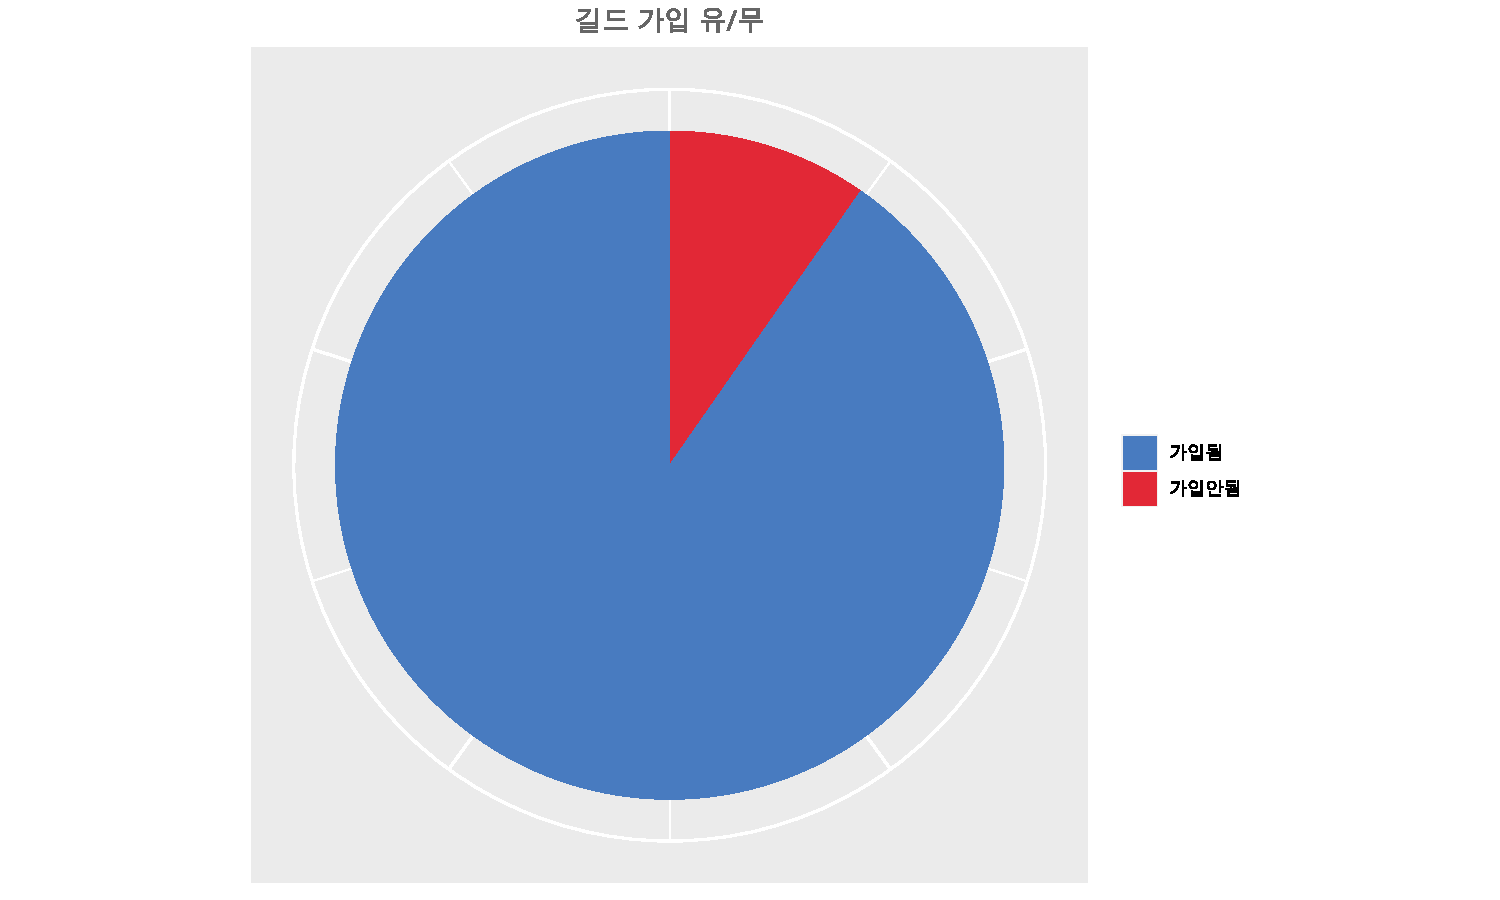
\includegraphics{123_files/figure-latex/ranking_all_guild-1.pdf}

\begin{longtable}[]{@{}cc@{}}
\toprule()
길드 가입안됨 & 길드 가입됨 \\
\midrule()
\endhead
4847(9.69\%) & 45413(90.9\%) \\
\bottomrule()
\end{longtable}

분석 결과 약 10\%의 인원만 가입하지 않았으며, 나머지는 모두 길드에
가입하였다. 이에 상위권은 대부분 길드에 가입되어있다는 사실을 알 수
있었다.

위 데이터로 길드의 유무도 실력 차에 영향을 끼치는 것을 알 수 있었다.

\hypertarget{uxc778uxae30uxb3c4uxc640-uxb7aduxd0b9uxc758-uxc0c1uxad00uxad00uxacc4}{%
\subsubsection{인기도와 랭킹의
상관관계}\label{uxc778uxae30uxb3c4uxc640-uxb7aduxd0b9uxc758-uxc0c1uxad00uxad00uxacc4}}

직업과 레벨간 편차에서 이용하지 않은 수치가 하나 있다. 바로
'인기도'인데, 이는 해당 사용자는 조정할 수 없으며, 다른 사용자가
인기도를 증감시킨다.

인기도는 예전에는 게임에 직접적인 영향을 끼치기도 했으나, 현재는 게임에
직접적인 영향을 끼치는 않는다.

다만, 250레벨 이상은 게임에서 특정 조건을 만족 시킬 때 게임에 영향을
끼치는 버프를 주는 경우가 있으므로\footnote{250/275레벨 이상 달성 시
  주는 의자에 앉아 있을 경우, 해당 캐릭터의 인기도를 상승시켰을 때
  30분의 공격력/마력 증가 버프 발현} 인기도가 높을 수 있다.

그렇다면 랭킹이 높을 수록 인기도가 높을 가능성이 높다는 가설이
수립되는데, 과연 그런지 파악해보기로 하였다.

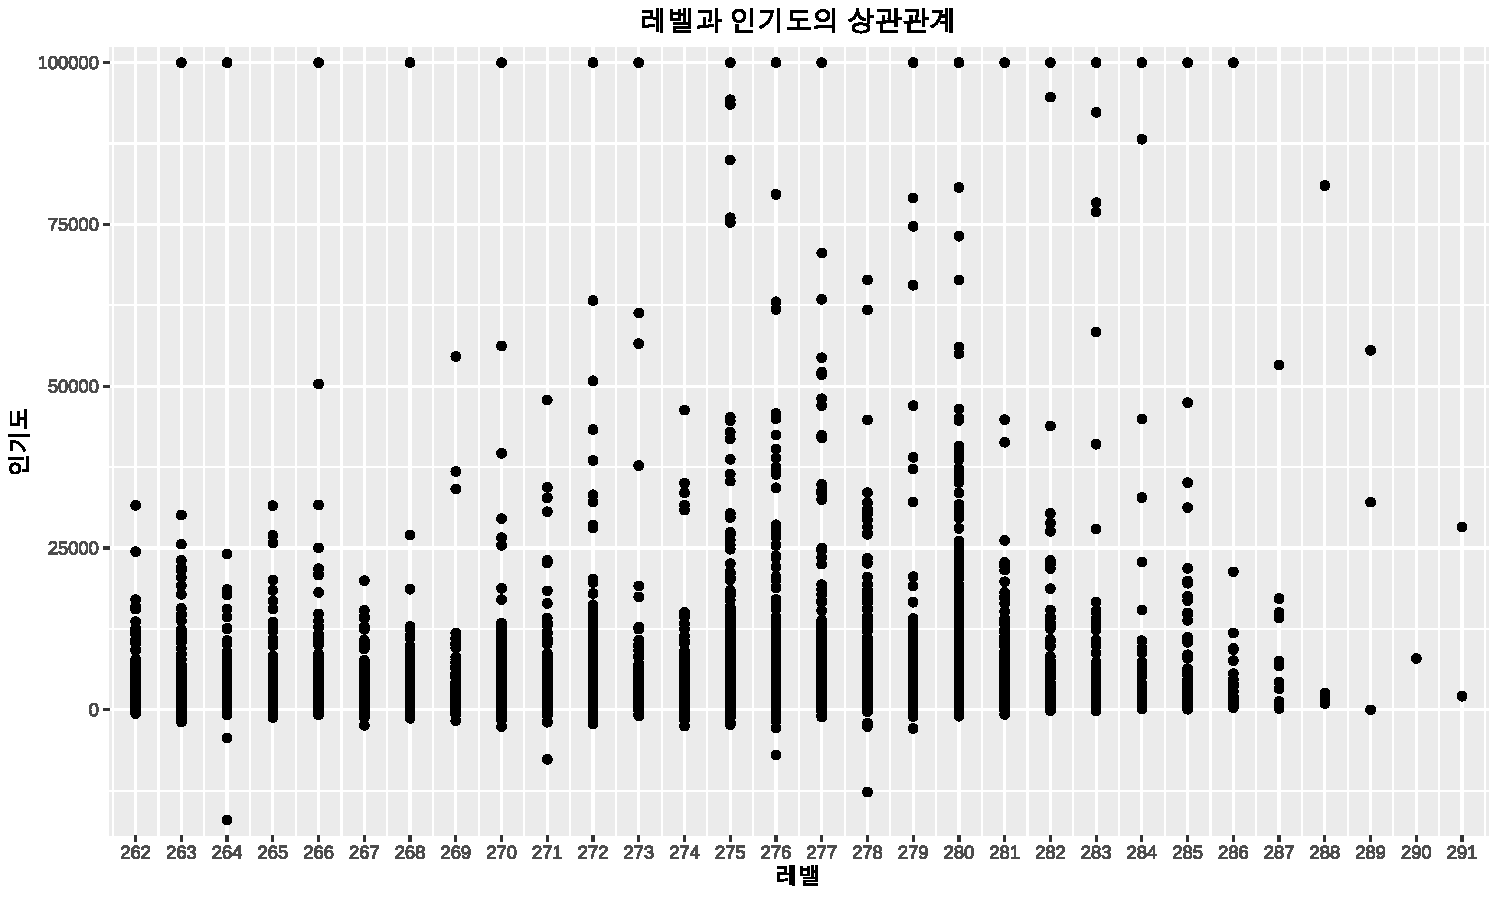
\includegraphics{123_files/figure-latex/ranking_all_inki-1.pdf}

인기도의 범위는 -99,999부터 99,999까지이다. 최하 인기도가 -17,005라
그래프를 잘랐다.

평균 인기도는 1065.90이다. 소숫점 2자리에서 반올림하였다.

그래프를 보면 알겠지만 대부분의 캐릭터는 인기도가 0에서 25,000 구간에
머물러있는것을 볼 수 있다. 또한 레벨이 높다고 인기도가 매우 높은 것도
아니고, 오히려 264레벨에서 인기도 최고치인 99,999가 관측되었다.

이로써 인기도와 랭킹의 상관관게는 없다고 볼 수 있다.

\hypertarget{uxc11cuxbc84-uxb7aduxd0b9}{%
\subsection{서버 랭킹}\label{uxc11cuxbc84-uxb7aduxd0b9}}

이제까지는 '통합 랭킹'에 관한 통계를 내보았다면, 이제는 각 서버별 랭킹을
알아보자.

'메이플스토리'에는 총 12개의 서버가 있다.\footnote{리부트 서버, 이벤트
  서버(버닝, 핑크빈 등) 제외} 각 서버는 별개로 취급되며, 캐릭터 및
아이템의 이동은 제한된다.\footnote{월드 리프(캐릭터), 레이디 블레어의
  드림 익스프레스 이벤트(캐시아이템) 한정 가능}

따라서 서버별로 인구 수, 직업 분포 등이 다를 것이므로, 이를
파악해봄으로써 '전체 랭킹'에서의 직업간 편차가 여기에서도 존재하는지
확인해보기로 하였다.

그리고 '서버간 격차'의 존재 유무도 파악해보기로 하였다.

\hypertarget{uxac01-uxc11cuxbc84uxbcc4-uxc9c1uxc5c5-uxbd84uxd3ec}{%
\subsubsection{각 서버별 직업
분포}\label{uxac01-uxc11cuxbc84uxbcc4-uxc9c1uxc5c5-uxbd84uxd3ec}}

먼저 '전체 랭킹'에서 하였던 것과 마찬가지로 각 서버 별 직업의 분포를
파악해보고자 하였다.

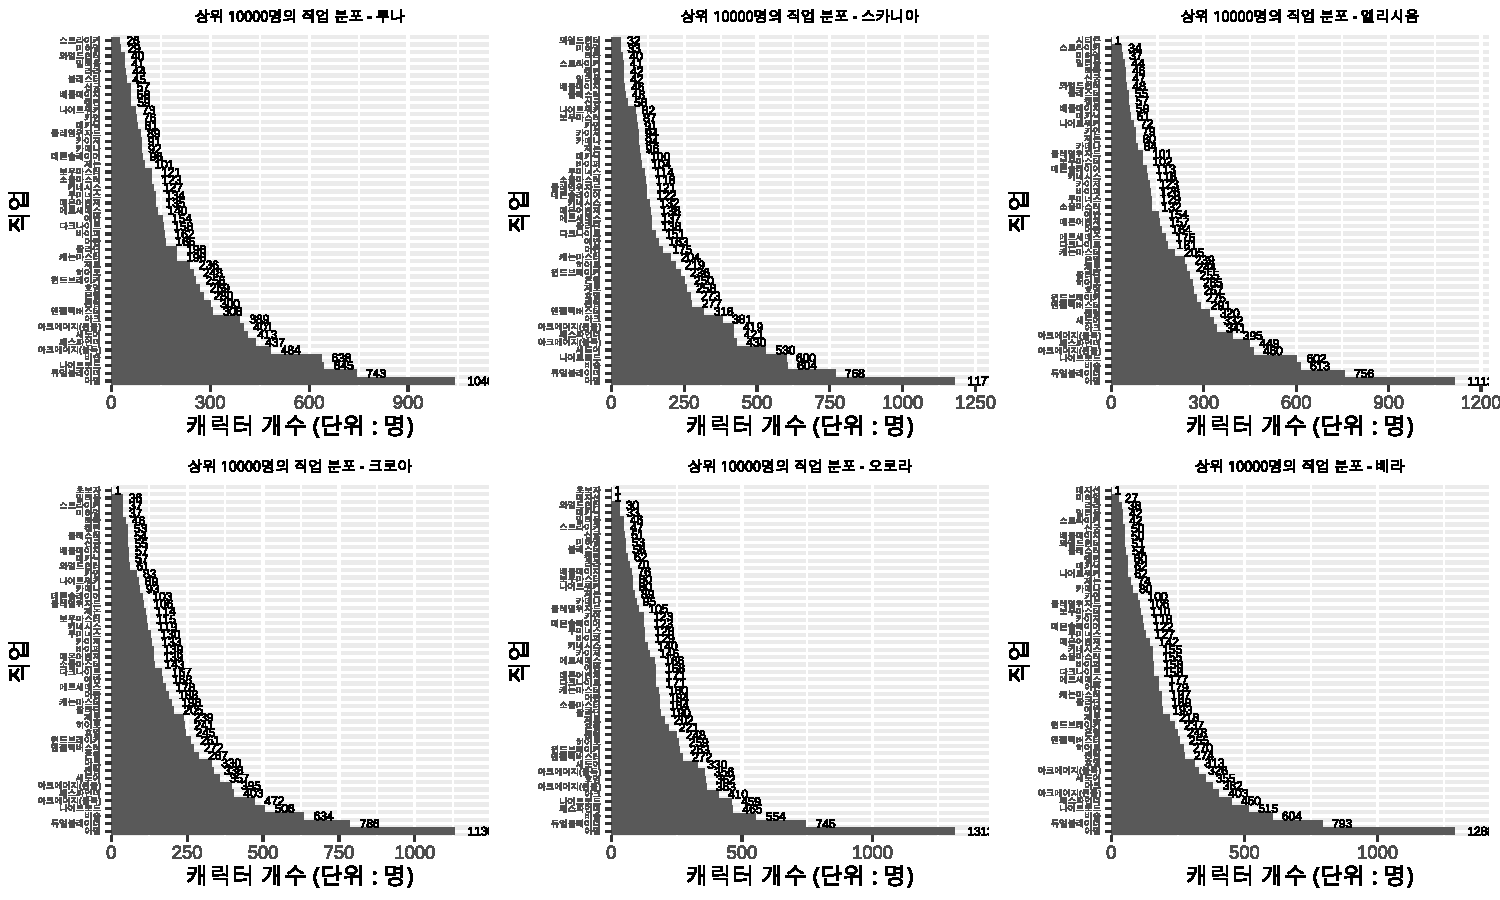
\includegraphics{123_files/figure-latex/ranking_server_job-1.pdf}
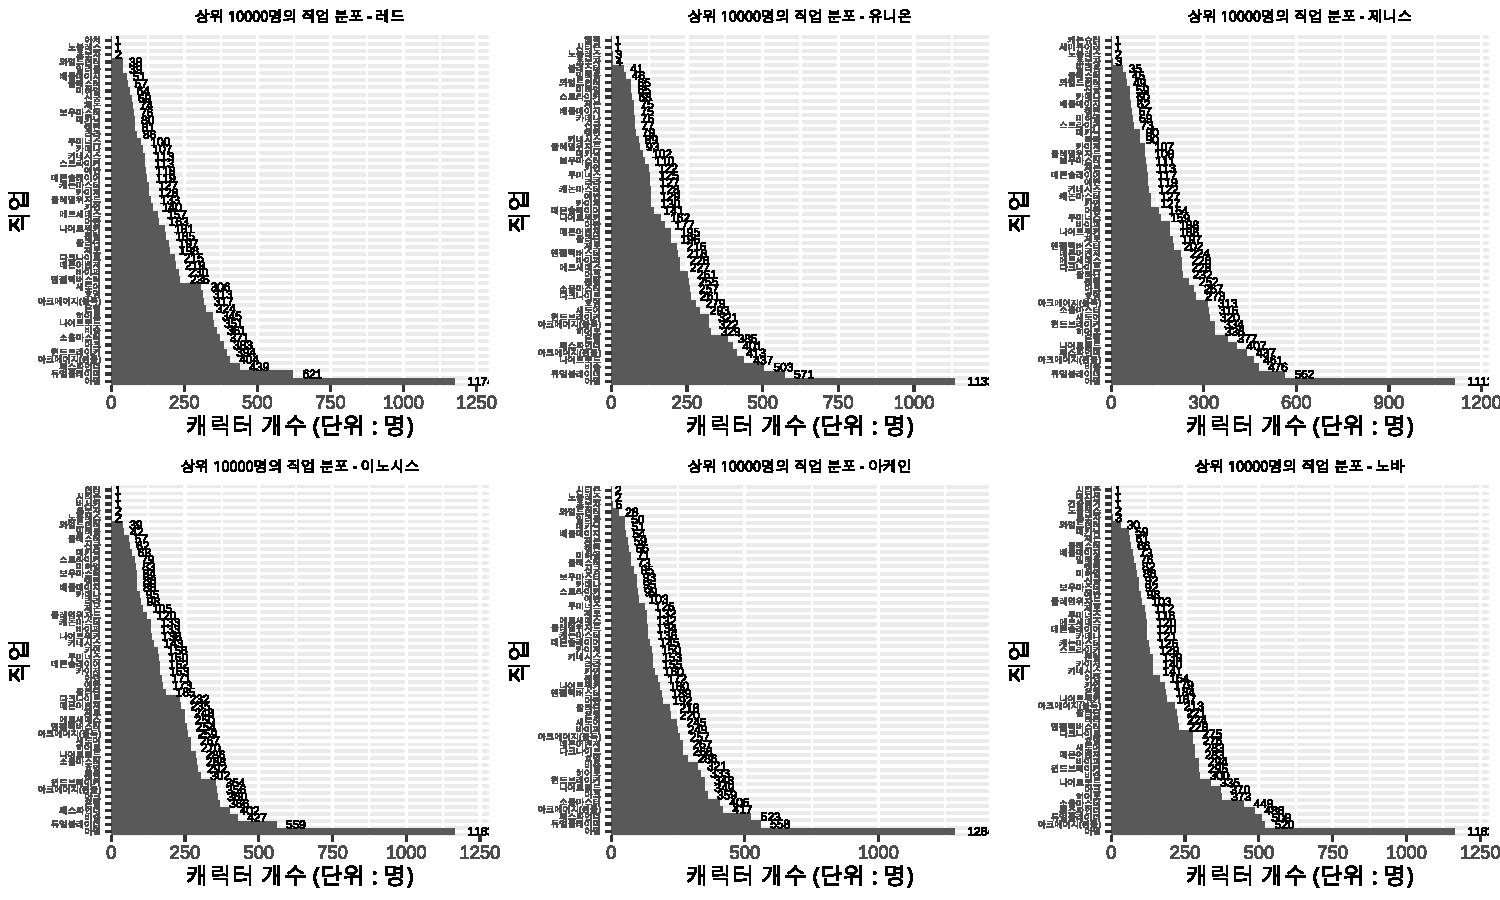
\includegraphics{123_files/figure-latex/ranking_server_job-2.pdf}

서버의 개수가 많음에 따라 간략하게 보기 위하여 서버별 상위 직업 3개와
하위 직업 3개를 따로 정리하였으며 이는 다음과 같다.

\begin{longtable}[]{@{}
  >{\raggedright\arraybackslash}p{(\columnwidth - 6\tabcolsep) * \real{0.0800}}
  >{\raggedright\arraybackslash}p{(\columnwidth - 6\tabcolsep) * \real{0.2960}}
  >{\raggedright\arraybackslash}p{(\columnwidth - 6\tabcolsep) * \real{0.2400}}
  >{\raggedright\arraybackslash}p{(\columnwidth - 6\tabcolsep) * \real{0.3840}}@{}}
\toprule()
\begin{minipage}[b]{\linewidth}\raggedright
서버
\end{minipage} & \begin{minipage}[b]{\linewidth}\raggedright
상위직업
\end{minipage} & \begin{minipage}[b]{\linewidth}\raggedright
하위직업
\end{minipage} & \begin{minipage}[b]{\linewidth}\raggedright
제외직업
\end{minipage} \\
\midrule()
\endhead
루나 & 아델,듀얼블레이더,나이트로드 & 스트라이커,미하일,와일드헌터 & \\
스카니아 & 아델,듀얼블레이더,비숍 & 와일드헌터,미하일,라라 & \\
엘리시움 & 아델,듀얼블레이더,비숍 & 스트라이커,미하일,일리움 &
시티즌\footnote{레지스탕스 계열 0차 전직 직업} \\
크로아 & 아델,듀얼블레이더,비숍 & 일리움,스트라이커,미하일 &
초보자\footnote{모험가 계열 0차 전직 직업} \\
오로라 & 아델,듀얼블레이더,비숍 & 와일드헌터,메카닉,일리움 & 초보자,
매지션\footnote{모험가(마법사)계열 1차 전직 직업} \\
베라 & 아델,듀얼블레이더,비숍 & 미하일,라라,일리움 & 매지션 \\
레드 & 아델,듀얼블레이더,패스파인더 & 와일드헌터,일리움,배틀메이지 &
아처\footnote{모험가(궁수)계열 1차 전직 직업}, 노블레스\footnote{시그너스
  기사단 계열 0차 전직 직업}, 초보자 \\
유니온 & 아델,듀얼블레이더,비숍 & 블래스터,일리움,와일드헌터 &
해적\footnote{모험가(해적)계열 1차 전직 직업},시티즌,노블레스,초보자 \\
제니스 & 아델,듀얼블레이더,비숍 & 일리움,블래스터,와일드헌터 &
캐논슈터\footnote{캐논마스터 2차 전직 직업}
,세미듀어러\footnote{듀얼블레이더 1.5차 전직 직업},노블레스,초보자 \\
이노시스 & 아델,듀얼블레이더,비숍 & 와일드헌터,일리움,블래스터 &
헌터\footnote{보우마스터 2차 전직 직업}
,시티즌,버서커\footnote{다크나이트 3차 전직 직업},노블레스,초보자 \\
아케인 & 아델,듀얼블레이더,패스파인더 & 와일드헌터,일리움,메카닉 &
시티즌,노블레스,초보자 \\
노바 & 아델,아크메이지(썬콜), 듀얼블레이더 & 와일드헌터,메카닉,제논 &
시티즌,매지션,건슬링거\footnote{캡틴 2차 전직 직업},노블레스,초보자 \\
\bottomrule()
\end{longtable}

대체적으로 `아델', `듀얼블레이더', `비숍'가 상위 3개 직업을 차지하였다.
또한 '나이트로드'나 '패스파인더', '아크메이지(썬콜)'이 상위 3개에 랭크된
경우도 있었다.

이들은 모두 '전체 랭킹'에서 1\textasciitilde7위를 기록하고 있다.

반대로 하위직업은 `와일드헌터', `미하일', `일리움'이 하위 3개 직업을
기록하였다. 간혹 '메카닉', `스트라이커', `블래스터' 등도 하위직업에
위치한 적이 있다.

이들은 대체로 '전체 랭킹'에서 40\textasciitilde45위를 기록하고 있다.
(제논 31위, 메카닉 36위, 배틀메이지 37위)

이를 조금 세부적으로 분석하기 위하여 각 서버에서 직업이 가지고 있는
순위를 모두 합산하여 평균을 내보았다. 정렬은 평균 순위로 하였다.

\begin{table}[H]
\centering
\resizebox{\linewidth}{!}{
\begin{tabular}{l|l|l|l|l|l|l|l|l|l|l|l|l|l}
\hline
직업 & 루나 & 스카니아 & 엘리시움 & 크로아 & 오로라 & 베라 & 레드 & 유니온 & 제니스 & 이노시스 & 아케인 & 노바 & 평균\\
\hline
아델 & \textcolor{blue}{\textbf{1}} & \textcolor{blue}{\textbf{1}} & \textcolor{blue}{\textbf{1}} & \textcolor{blue}{\textbf{1}} & \textcolor{blue}{\textbf{1}} & \textcolor{blue}{\textbf{1}} & \textcolor{blue}{\textbf{1}} & \textcolor{blue}{\textbf{1}} & \textcolor{blue}{\textbf{1}} & \textcolor{blue}{\textbf{1}} & \textcolor{blue}{\textbf{1}} & \textcolor{blue}{\textbf{1}} & \textcolor{blue}{\textbf{1}}\\
\hline
듀얼블레이더 & \textbf{2} & \textbf{2} & \textbf{2} & \textbf{2} & \textbf{2} & \textbf{2} & \textbf{2} & \textbf{2} & \textbf{2} & \textbf{2} & \textbf{2} & \textbf{3} & \textbf{2.08}\\
\hline
비숍 & \textbf{4} & \textbf{3} & \textbf{3} & \textbf{3} & \textbf{3} & \textbf{3} & 8 & \textbf{3} & \textbf{3} & \textbf{3} & 10 & 9 & \textbf{4.58}\\
\hline
패스파인더 & 6 & 7 & 6 & 6 & \textbf{4} & \textbf{5} & \textbf{3} & 6 & \textbf{5} & \textbf{4} & \textbf{3} & \textbf{4} & \textbf{4.92}\\
\hline
아크메이지(썬콜) & 8 & 8 & \textbf{5} & 7 & 7 & 6 & \textbf{4} & \textbf{5} & \textbf{4} & 7 & \textbf{4} & \textbf{2} & \textbf{5.58}\\
\hline
나이트로드 & \textbf{3} & \textbf{4} & \textbf{4} & \textbf{4} & \textbf{5} & \textbf{4} & 9 & \textbf{4} & 6 & 12 & 7 & 8 & \textbf{5.83}\\
\hline
아크 & 9 & 9 & 8 & 10 & 6 & 7 & 6 & 16 & 14 & 6 & 6 & 7 & 8.67\\
\hline
아크메이지(불독) & \textbf{5} & 6 & 7 & \textbf{5} & 9 & 9 & 12 & 9 & 12 & 15 & 14 & 19 & 10.17\\
\hline
섀도어 & 7 & \textbf{5} & 9 & 8 & 10 & 8 & 14 & 11 & 10 & 14 & 16 & 12 & 10.33\\
\hline
윈드브레이커 & 14 & 15 & 12 & 13 & 12 & 15 & \textbf{5} & 10 & 9 & 8 & 8 & 10 & 10.92\\
\hline
히어로 & 15 & 16 & 14 & 15 & 13 & 12 & 10 & 8 & 8 & 13 & 9 & 6 & 11.58\\
\hline
호영 & 13 & 12 & 13 & 14 & 8 & 10 & 13 & 12 & 13 & 10 & 11 & 14 & 11.92\\
\hline
은월 & 12 & 14 & 17 & 11 & 15 & 14 & 11 & 7 & 7 & \textbf{5} & 17 & 21 & 12.58\\
\hline
엔젤릭버스터 & 10 & 10 & 11 & 12 & 11 & 13 & 15 & 19 & 20 & 16 & 20 & 16 & 14.42\\
\hline
팬텀 & 11 & 11 & 10 & 9 & 14 & 11 & 21 & 15 & 15 & 9 & 22 & 26 & 14.5\\
\hline
소울마스터 & 27 & 27 & 24 & 23 & 18 & 24 & 7 & 14 & 11 & 11 & \textbf{5} & \textbf{5} & 16.33\\
\hline
팔라딘 & 17 & 21 & 15 & 17 & 17 & 18 & 20 & 21 & 16 & 21 & 18 & 18 & 18.25\\
\hline
다크나이트 & 21 & 20 & 19 & 22 & 21 & 22 & 18 & 13 & 17 & 20 & 12 & 15 & 18.33\\
\hline
제로 & 16 & 13 & 16 & 16 & 16 & 16 & 19 & 20 & 21 & 18 & 30 & 33 & 19.5\\
\hline
데몬어벤져 & 24 & 23 & 22 & 24 & 21 & 26 & 17 & 22 & 19 & 19 & 13 & 12 & 20.17\\
\hline
아란 & 19 & 18 & 21 & 19 & 18 & 20 & 23 & 23 & 25 & 23 & 19 & 23 & 20.92\\
\hline
바이퍼 & 20 & 29 & 26 & 24 & 27 & 22 & 16 & 18 & 22 & 30 & 15 & 11 & 21.67\\
\hline
메르세데스 & 23 & 22 & 20 & 20 & 24 & 21 & 24 & 17 & 17 & 17 & 30 & 30 & 22.08\\
\hline
캐논마스터 & 17 & 17 & 18 & 18 & 20 & 19 & 28 & 28 & 26 & 30 & 28 & 28 & 23.08\\
\hline
에반 & 22 & 19 & 23 & 21 & 23 & 17 & 30 & 27 & 29 & 22 & 33 & 35 & 25.08\\
\hline
키네시스 & 26 & 24 & 28 & 28 & 26 & 24 & 31 & 35 & 28 & 28 & 25 & 24 & 27.25\\
\hline
카이저 & 32 & 32 & 27 & 26 & 25 & 29 & 27 & 26 & 34 & 24 & 26 & 25 & 27.75\\
\hline
루미너스 & 25 & 28 & 25 & 27 & 28 & 27 & 34 & 30 & 24 & 26 & 32 & 32 & 28.17\\
\hline
데몬슬레이어 & 30 & 25 & 29 & 32 & 29 & 28 & 29 & 25 & 30 & 25 & 27 & 30 & 28.25\\
\hline
나이트워커 & 36 & 36 & 35 & 34 & 34 & 35 & 22 & 24 & 22 & 29 & 21 & 20 & 29\\
\hline
카인 & 35 & 34 & 34 & 35 & 29 & 32 & 25 & 31 & 26 & 27 & 23 & 22 & 29.42\\
\hline
플레임위자드 & 33 & 26 & 31 & 31 & 31 & 31 & 26 & 34 & 33 & 32 & 29 & 34 & 30.92\\
\hline
보우마스터 & 28 & 35 & 30 & 29 & 34 & 30 & 38 & 32 & 32 & 38 & 36 & 36 & 33.17\\
\hline
카데나 & 31 & 32 & 32 & 33 & 32 & 33 & 33 & 38 & \textbf{41} & 35 & 35 & 29 & 33.67\\
\hline
제논 & 29 & 31 & 33 & 30 & 33 & 34 & 39 & 39 & 31 & 33 & \textbf{41} & \textbf{43} & 34.67\\
\hline
라라 & \textbf{41} & \textbf{43} & \textbf{42} & \textbf{42} & 37 & \textbf{44} & 35 & 29 & 35 & 34 & 24 & 17 & 35.25\\
\hline
메카닉 & 34 & 30 & 36 & 37 & \textbf{44} & 35 & 37 & 33 & 35 & \textbf{41} & \textbf{43} & \textbf{44} & 37.42\\
\hline
캡틴 & 37 & 40 & 38 & \textbf{41} & 38 & 37 & 36 & 36 & 39 & 36 & 40 & 39 & 38.08\\
\hline
배틀메이지 & 38 & 39 & 37 & 37 & 36 & 40 & \textbf{43} & 39 & 40 & 36 & \textbf{42} & \textbf{41} & 39\\
\hline
스트라이커 & \textcolor{red}{\textbf{45}} & \textbf{42} & \textcolor{red}{\textbf{45}} & \textbf{43} & \textbf{42} & \textbf{42} & 31 & \textbf{41} & 37 & 40 & 34 & 27 & 39.08\\
\hline
신궁 & 39 & 37 & \textbf{41} & 39 & \textbf{41} & 40 & 40 & 37 & \textbf{42} & \textbf{42} & 37 & 36 & 39.25\\
\hline
블래스터 & 40 & 38 & 39 & 40 & 39 & 38 & \textbf{42} & \textcolor{red}{\textbf{45}} & \textbf{44} & \textbf{43} & 38 & \textbf{42} & \textbf{40.67}\\
\hline
미하일 & \textbf{44} & \textbf{44} & \textbf{44} & \textbf{43} & 40 & \textcolor{red}{\textbf{45}} & \textbf{41} & \textbf{42} & 38 & 39 & 39 & 38 & \textbf{41.42}\\
\hline
와일드헌터 & \textbf{43} & \textcolor{red}{\textbf{45}} & 40 & 36 & \textcolor{red}{\textbf{45}} & 39 & \textcolor{red}{\textbf{45}} & \textbf{42} & \textbf{43} & \textcolor{red}{\textbf{45}} & \textcolor{red}{\textbf{45}} & \textcolor{red}{\textbf{45}} & \textbf{42.75}\\
\hline
일리움 & \textbf{42} & 40 & \textbf{43} & \textcolor{red}{\textbf{45}} & \textbf{43} & \textbf{42} & \textbf{44} & \textbf{44} & \textcolor{red}{\textbf{45}} & \textbf{44} & \textbf{44} & 40 & \textcolor{red}{\textbf{43}}\\
\hline
\end{tabular}}
\end{table}

이런 도중에 메이플스토리 관련 커뮤니티에서는 '서버의 서열화'가
이루어졌다. 일명 '도시서버'와 '시골서버'인데, 월드 리프 제한을 기점으로
나누게 된다. 위 서버를 분류하자면 이렇게 된다.

\begin{itemize}
\item
  도시서버 : 루나, 스카니아, 엘리시움, 크로아, 베라
\item
  시골서버 : 오로라, 레드, 유니온, 제니스, 이노시스, 아케인, 노바
\end{itemize}

이 '서열화된 서버'를 기준으로 한번 분석해보았을 때, 분석 결과는 다음과
같다.

\begin{itemize}
\item
  `전체 랭킹' 상위 5개 직업과 비교했을 때 '패스파인더'가 들어오고,
  '나이트로드'가 6위로 밀렸다. (전체 랭킹에서 패스파인더는 6위였다.)

  \begin{itemize}
  \tightlist
  \item
    '나이트로드'는 '도시 서버'에서 높은 순위를 얻은 반면, '시골
    서버'에서는 순위가 낮아졌다. 반대로 '패스파인더'는 뒷서버에서는
    순위가 높았다.
  \end{itemize}
\item
  또한 `소울마스터'가 '아케인', '노바'에서 상위 5개 직업에 랭크되었다.
  (전체 랭킹 25위)
\item
  `전체 랭킹' 하위 5개 직업과 비교했을 때 `스트라이커', `라라'가 빠지고
  '신궁', '블래스터'가 들어왔다. (신궁 전체 랭킹 38위, 블래스터 전체
  랭킹 40위)

  \begin{itemize}
  \tightlist
  \item
    '라라'는 '도시 서버'에서 하위권에 랭크되었으나 '시골 서버'에서 최고
    순위 17위까지 기록하는 등 약진을 이루었다.
  \item
    '스트라이커'도 '시골 서버'에서 27위를 기록하는 등 '앞서버'도시
    서버'와 차이가 있다.
  \item
    `신궁', '블래스터'는 '도시 서버'와 '시골 서버'에서 모두 하위권에
    랭크되어 하위 5개 직업으로 내려갔다.
  \end{itemize}
\item
  전체적으로 '전체 랭킹'과 비교하였을 때 '도시 서버'는 비슷한 순위를
  가진 반면, '시골 서버'는 약간의 차이가 있는 것을 볼 수 있다.

  \begin{itemize}
  \tightlist
  \item
    특히 '아케인'과 '노바'가 그러한 경향이 심한 걸 볼 수 있다.
  \end{itemize}
\end{itemize}

'전체 랭킹'의 표본이 50,000명이었고, '서버 랭킹'의 표본은 10,000*12 =
120,000명이었다. '도시 서버'가 전체 랭킹과 비슷하다는 것은 '도시 서버'가
전체 랭킹에 조금 더 많이 포진되어있었다고 결론내릴 수 있다. 이에
서버간에도 편차가 존재한다는 사실을 확인할 수 있었다.

\hypertarget{uxcc28-uxc804uxc9c1uxc774-uxc544uxb2cc-uxc0c1uxc704uxb7aduxcee4}{%
\paragraph{4차 전직이 아닌
상위랭커}\label{uxcc28-uxc804uxc9c1uxc774-uxc544uxb2cc-uxc0c1uxc704uxb7aduxcee4}}

※ 수행평가 항목 : sqldf 사용 및 응용

근데 이 것을 정리하다가 의문점이 들었다. 바로 4차 전직 미만인 직업들이
상위 랭킹에 기록된 경우이다. 실제로 위 표의 '제외 직업'에는 0차부터
3차까지 고르게 분포되어있는 모습을 볼 수 있었다. 이러한 경우는 특수한
경우이므로 따로 통계를 내보려고 한다.

\begin{Shaded}
\begin{Highlighting}[]
\NormalTok{result }\OtherTok{\textless{}{-}} \FunctionTok{data.frame}\NormalTok{(}\FunctionTok{matrix}\NormalTok{(}\AttributeTok{ncol =} \DecValTok{2}\NormalTok{, }\AttributeTok{nrow =} \DecValTok{0}\NormalTok{))}
\FunctionTok{colnames}\NormalTok{(result) }\OtherTok{\textless{}{-}} \FunctionTok{c}\NormalTok{(}\StringTok{"level"}\NormalTok{, }\StringTok{"job"}\NormalTok{)}
\NormalTok{server }\OtherTok{=} \FunctionTok{list}\NormalTok{(}\StringTok{"luna"}\NormalTok{, }\StringTok{"scania"}\NormalTok{, }\StringTok{"elysium"}\NormalTok{, }\StringTok{"croa"}\NormalTok{, }\StringTok{"aurora"}\NormalTok{, }\StringTok{"bera"}\NormalTok{, }\StringTok{"red"}\NormalTok{, }\StringTok{"\textquotesingle{}union\textquotesingle{}"}\NormalTok{, }\StringTok{"zenith"}\NormalTok{, }\StringTok{"enosis"}\NormalTok{, }\StringTok{"arcane"}\NormalTok{, }\StringTok{"nova"}\NormalTok{)}
\NormalTok{job }\OtherTok{=} \FunctionTok{list}\NormalTok{(}\StringTok{"시티즌"}\NormalTok{, }\StringTok{"초보자"}\NormalTok{, }\StringTok{"매지션"}\NormalTok{, }\StringTok{"아처"}\NormalTok{, }\StringTok{"노블레스"}\NormalTok{, }\StringTok{"해적"}\NormalTok{, }\StringTok{"캐논슈터"}\NormalTok{, }\StringTok{"세미듀어러"}\NormalTok{, }\StringTok{"헌터"}\NormalTok{, }\StringTok{"버서커"}\NormalTok{, }\StringTok{"건슬링거"}\NormalTok{)}
\ControlFlowTok{for}\NormalTok{ (i }\ControlFlowTok{in}\NormalTok{ job) \{}
  \ControlFlowTok{for}\NormalTok{ (j }\ControlFlowTok{in}\NormalTok{ server) \{}
\NormalTok{    string }\OtherTok{\textless{}{-}} \FunctionTok{paste}\NormalTok{(}\StringTok{"select level, job from"}\NormalTok{, j, }\FunctionTok{paste}\NormalTok{(}\StringTok{"where job =}\SpecialCharTok{\textbackslash{}\textquotesingle{}}\StringTok{"}\NormalTok{, i, }\StringTok{"}\SpecialCharTok{\textbackslash{}\textquotesingle{}}\StringTok{"}\NormalTok{, }\AttributeTok{sep=}\StringTok{\textquotesingle{}\textquotesingle{}}\NormalTok{))}
\NormalTok{    result }\OtherTok{\textless{}{-}} \FunctionTok{rbind}\NormalTok{(result, }\FunctionTok{sqldf}\NormalTok{(string))}
\NormalTok{  \}}
\NormalTok{\}}

\NormalTok{result2 }\OtherTok{\textless{}{-}} \FunctionTok{data.frame}\NormalTok{(}\FunctionTok{matrix}\NormalTok{(}\AttributeTok{ncol =} \DecValTok{4}\NormalTok{, }\AttributeTok{nrow =} \DecValTok{0}\NormalTok{))}
\FunctionTok{colnames}\NormalTok{(result2) }\OtherTok{\textless{}{-}} \FunctionTok{c}\NormalTok{(}\StringTok{"job"}\NormalTok{, }\StringTok{"min"}\NormalTok{, }\StringTok{"max"}\NormalTok{, }\StringTok{"mean"}\NormalTok{)}
\ControlFlowTok{for}\NormalTok{ (i }\ControlFlowTok{in}\NormalTok{ job) \{}
\NormalTok{  temp }\OtherTok{\textless{}{-}} \FunctionTok{data.frame}\NormalTok{(}\FunctionTok{matrix}\NormalTok{(}\AttributeTok{ncol =} \DecValTok{2}\NormalTok{, }\AttributeTok{nrow =} \DecValTok{0}\NormalTok{))}
  \FunctionTok{colnames}\NormalTok{(temp) }\OtherTok{\textless{}{-}} \FunctionTok{c}\NormalTok{(}\StringTok{"level"}\NormalTok{, }\StringTok{"job"}\NormalTok{)}
\NormalTok{  string }\OtherTok{\textless{}{-}} \FunctionTok{paste}\NormalTok{(}\StringTok{"select level, job from result where job=}\SpecialCharTok{\textbackslash{}\textquotesingle{}}\StringTok{"}\NormalTok{,i,}\StringTok{"}\SpecialCharTok{\textbackslash{}\textquotesingle{}}\StringTok{"}\NormalTok{, }\AttributeTok{sep=}\StringTok{\textquotesingle{}\textquotesingle{}}\NormalTok{)}
\NormalTok{  temp }\OtherTok{\textless{}{-}} \FunctionTok{rbind}\NormalTok{(temp, }\FunctionTok{sqldf}\NormalTok{(string))}
\NormalTok{  result2[}\FunctionTok{nrow}\NormalTok{(result2) }\SpecialCharTok{+} \DecValTok{1}\NormalTok{,] }\OtherTok{\textless{}{-}} \FunctionTok{list}\NormalTok{(i, }\FunctionTok{min}\NormalTok{(temp}\SpecialCharTok{$}\NormalTok{level), }\FunctionTok{max}\NormalTok{(temp}\SpecialCharTok{$}\NormalTok{level), }\FunctionTok{mean}\NormalTok{(temp}\SpecialCharTok{$}\NormalTok{level))}
\NormalTok{\}}

\FunctionTok{kable}\NormalTok{(result2, }\AttributeTok{col.names=}\FunctionTok{c}\NormalTok{(}\StringTok{"직업"}\NormalTok{, }\StringTok{"최소"}\NormalTok{, }\StringTok{"최대"}\NormalTok{, }\StringTok{"평균"}\NormalTok{)) }\SpecialCharTok{\%\textgreater{}\%}
  \FunctionTok{kable\_paper}\NormalTok{() }\SpecialCharTok{\%\textgreater{}\%}
  \FunctionTok{kable\_styling}\NormalTok{(}\AttributeTok{latex\_options =} \StringTok{"HOLD\_position"}\NormalTok{, }\AttributeTok{full\_width =} \ConstantTok{TRUE}\NormalTok{)}
\end{Highlighting}
\end{Shaded}

\begin{table}[H]
\centering
\begin{tabu} to \linewidth {>{\raggedright}X>{\raggedleft}X>{\raggedleft}X>{\raggedleft}X}
\hline
직업 & 최소 & 최대 & 평균\\
\hline
시티즌 & 222 & 261 & 246.3333\\
\hline
초보자 & 225 & 261 & 248.5238\\
\hline
매지션 & 230 & 260 & 249.3333\\
\hline
아처 & 258 & 258 & 258.0000\\
\hline
노블레스 & 222 & 261 & 244.7500\\
\hline
해적 & 251 & 251 & 251.0000\\
\hline
캐논슈터 & 242 & 242 & 242.0000\\
\hline
세미듀어러 & 244 & 244 & 244.0000\\
\hline
헌터 & 244 & 244 & 244.0000\\
\hline
버서커 & 252 & 252 & 252.0000\\
\hline
건슬링거 & 226 & 226 & 226.0000\\
\hline
\end{tabu}
\end{table}

먼저 0차 전직 직업이다.

\begin{itemize}
\item
  \textbf{시티즌}은 레지스탕스 계열 0차 전직 직업이다. 전체 서버에서
  6명이 존재했다. 최고 레벨은 261레벨이다.
\item
  \textbf{초보자}는 모험가 계열 0차 전직 직업이다. 전체 서버에서 21명이
  존재했다. 최고 레벨은 261레벨이다.
\end{itemize}

0차 전직 직업은 캐릭터가 처음 생성되었을 때 부여되는 직업이다. 일부
직업은 캐릭터 튜토리얼을 진행하면서 1차 전직을 완료하기에 0차 전직이
존재하지 않는 캐릭터도 있다. 스킬 및 대부분의 게임 기능을 사용하기
어렵기 때문에 하기 어려우나, 이러한 어려운 난이도 덕분에 일부러
초보자로만 육성하는 사람들이 있다. 그래서인지 가장 많은 캐릭터 수 (합
27명)이 도출되었다.

다음은 1차 전직 직업이다. (1.5차 직업 포함)

\begin{itemize}
\item
  \textbf{매지션}은 모험가(마법사) 계열 1차 전직 직업이다. 전체 서버에서
  3명이 존재했다. 최고 레벨은 260레벨이다.
\item
  \textbf{아처}는 모험가(궁수) 계열 1차 전직 직업이다. 전체 서버에서
  1명이 존재했다. 레벨은 258레벨이다.
\item
  \textbf{해적}은 모험가(해적) 계열 1차 전직 직업이다. 전체 서버에서
  1명이 존재했다. 레벨은 251레벨이다.
\item
  \textbf{세미듀어러}는 듀얼블레이더의 1.5차 전직 직업이다. 전체
  서버에서 1명이 존재했다. 레벨은 244레벨이다.
\end{itemize}

1차 전직구간은 0차 전직 직업보다는 많은 기능이 해금된다. 듀얼블레이더는
타 직업 대비 전직을 2번 더 하기에\footnote{총 6번. 타 직업은 4번한다.}
1.5차 전직이 있다. 1.5차 전직 구간은 20레벨부터 30레벨이다.

다음은 2차\textasciitilde3차 전직 직업이다.

\begin{itemize}
\item
  \textbf{캐논슈터}는 캐논마스터의 2차 전직 직업이다. 전체 서버에서
  1명이 존재했다. 레벨은 242레벨이다.
\item
  \textbf{헌터}는 보우마스터의 2차 전직 직업이다. 전체 서버에서 1명이
  존재했다. 레벨은 244레벨이다.
\item
  \textbf{건슬링거}는 다크나이트의 3차 전직 직업이다. 전체 서버에서
  1명이 존재했다. 레벨은 226레벨이다.
\end{itemize}

2차에서 3차 전직 직업은 1차 전직 대비 많은 기능이 해금된다.

여담으로, '전체 랭킹'의 50,000위의 랭킹이 262레벨이었다.\footnote{maple.gg
  기준 55,493위까지 262레벨이었다. 이번 프로젝트에서 사용된 자료에
  포함하지는 않았다.} 초보자/시티즌의 랭킹이 261레벨이었으니, 만약 조금
늦게 해당 프로젝트를 시작했으면 '전체 랭킹'에도 초보자/시티즌이 나올 수
있지 않았을까라는 생각을 가진다.

\hypertarget{uxac01-uxc11cuxbc84uxbcc4-uxb808uxbca8-uxbd84uxd3ec}{%
\subsubsection{각 서버별 레벨
분포}\label{uxac01-uxc11cuxbc84uxbcc4-uxb808uxbca8-uxbd84uxd3ec}}

'각 서버별 직업 분포'에서 우리는 서버별 편차가 존재한다는 것을 알 수
있었다. 그러나 정확히 얼마만큼의 차이가 존재하는지에 관해서는 알 수
없었기에, '전체 랭킹'에서 했던 것과 마찬가지로 비교적 객관적인 수치인
'레벨'을 이용하여 분석해보았다.

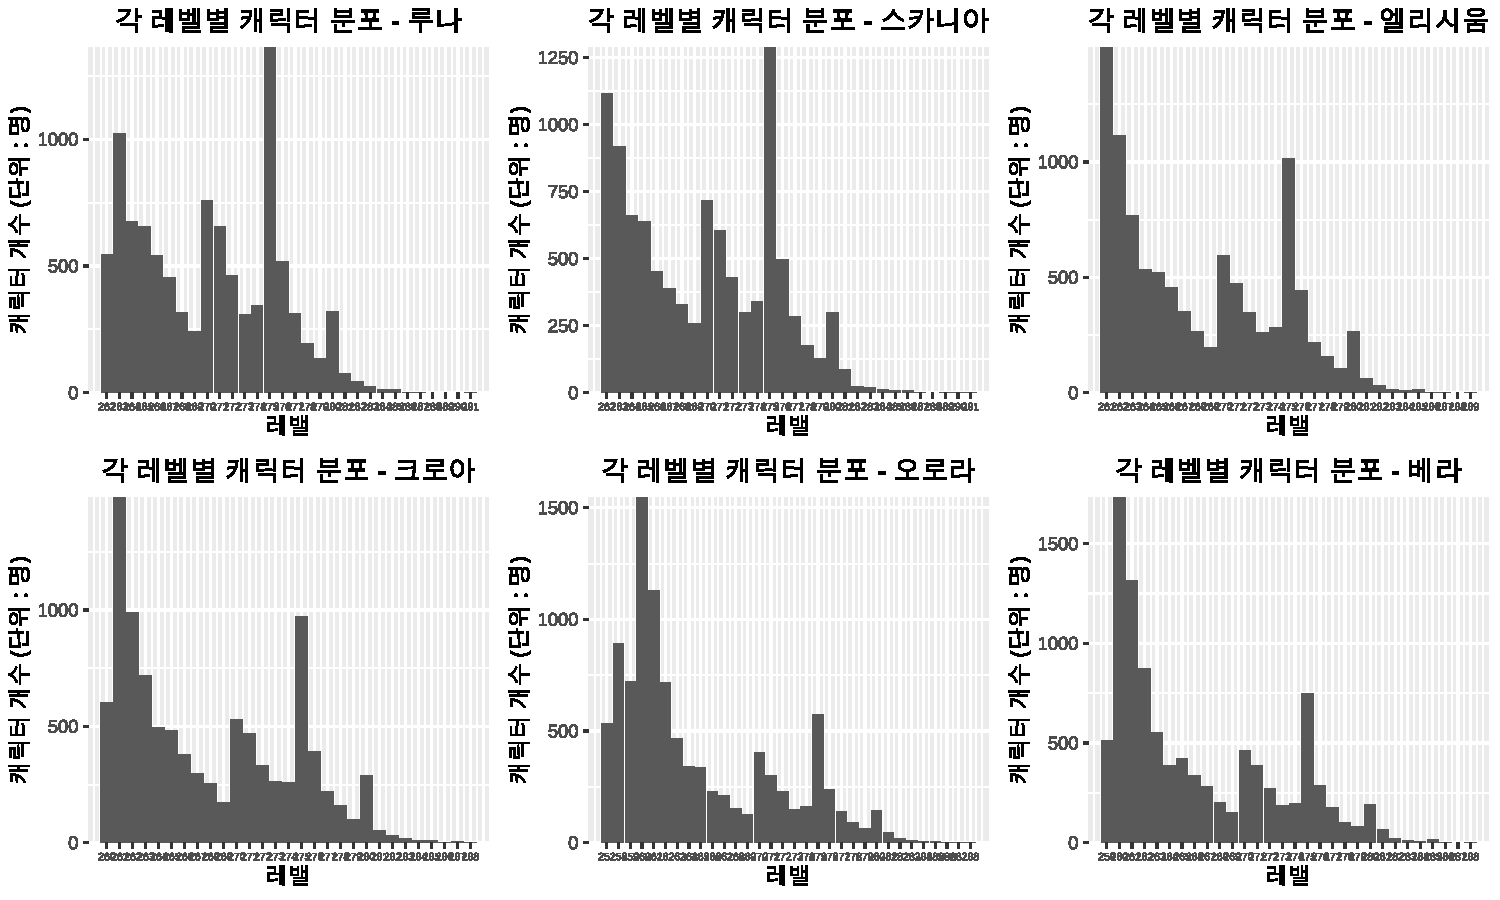
\includegraphics{123_files/figure-latex/ranking_server_level-1.pdf}
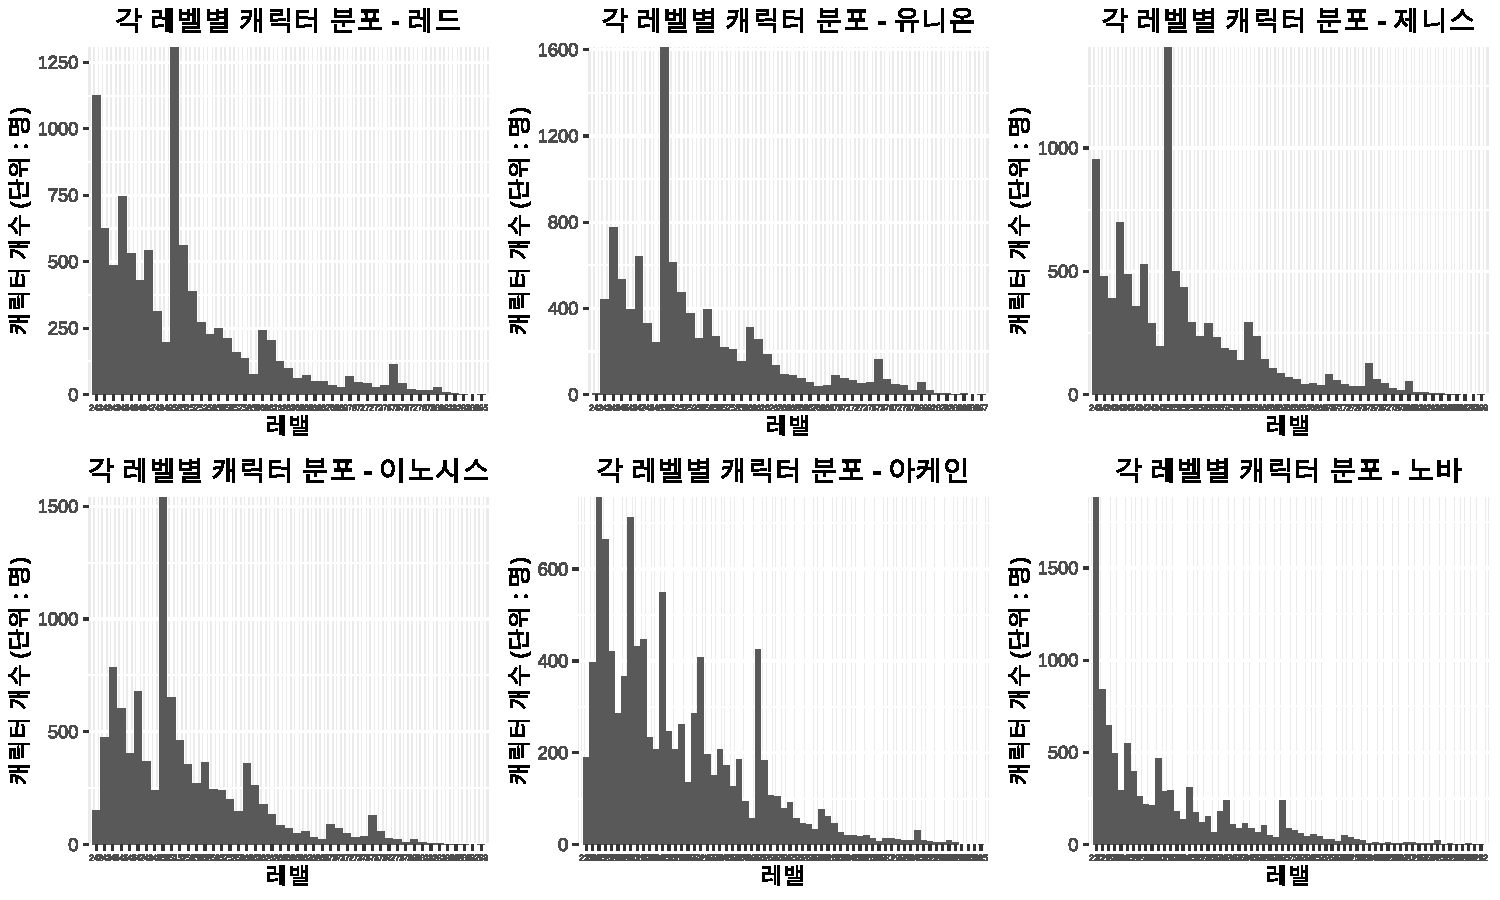
\includegraphics{123_files/figure-latex/ranking_server_level-2.pdf}

한눈에 수치들을 비교기 위하여 위 데이터들을 가지고 각 레벨 별로
통합하였다.

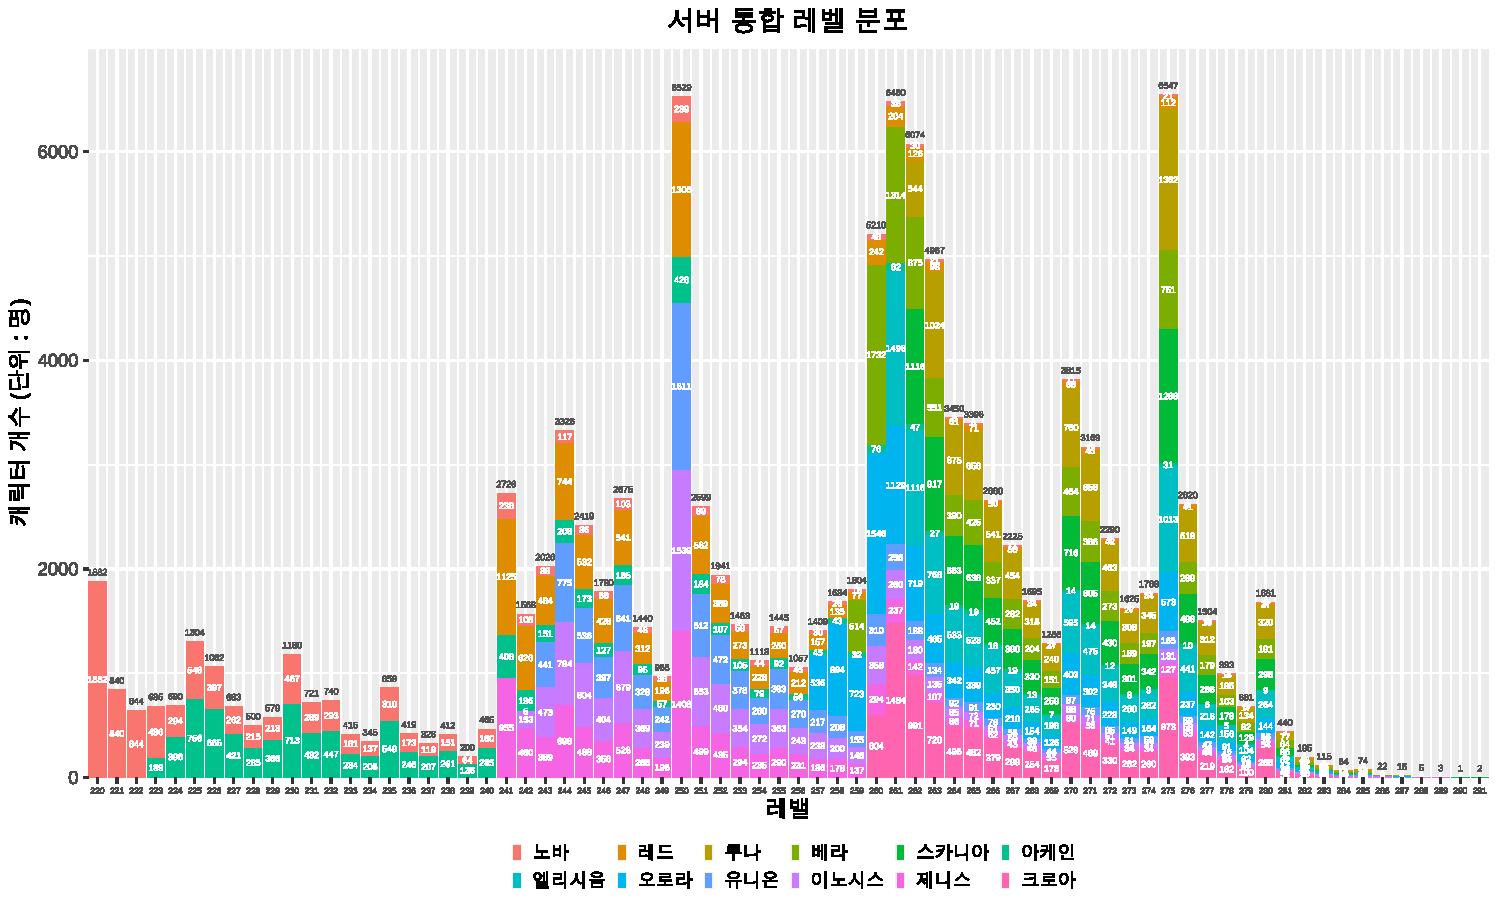
\includegraphics{123_files/figure-latex/ranking_server_job_3-1.pdf}

정확한 수치로 이를 파악하기 이위해 각 서버의 최대레벨, 최소레벨, 최빈값,
평균을 따로 정리하였다. 정렬은 평균레벨 순이다.

\begin{table}[H]
\centering
\begin{tabular}{l|l|l|l|l}
\hline
서버 & 최대레벨 & 최소레벨 & 최빈값 & 평균\\
\hline
루나 & \textcolor{red}{\textbf{291}} & \textcolor{red}{\textbf{262}} & \textcolor{red}{\textbf{275}} & \textcolor{red}{\textbf{270.08}}\\
\hline
스카니아 & \textcolor{red}{\textbf{291}} & \textcolor{red}{\textbf{262}} & \textcolor{red}{\textbf{275}} & 269.63\\
\hline
엘리시움 & 289 & 261 & 261 & 268.17\\
\hline
크로아 & 288 & 260 & 261 & 267.76\\
\hline
베라 & 288 & 259 & 260 & 266.11\\
\hline
오로라 & 288 & 257 & 260 & 264.5\\
\hline
유니온 & 287 & 242 & 250 & 253.24\\
\hline
이노시스 & 288 & 242 & 250 & 252.4\\
\hline
제니스 & 289 & 241 & 250 & 251.37\\
\hline
레드 & 285 & 241 & 250 & 250.2\\
\hline
아케인 & 285 & 223 & 225 & 236.65\\
\hline
노바 & \textcolor{blue}{\textbf{282}} & \textcolor{blue}{\textbf{220}} & \textcolor{blue}{\textbf{220}} & \textcolor{blue}{\textbf{230.39}}\\
\hline
\end{tabular}
\end{table}

분석 결과는 다음과 같다 :

\begin{itemize}
\item
  '도시서버'가 정확히 상위 5개 서버에 있다.

  \begin{itemize}
  \item
    '도시서버'는 대부분 평균 레벨이 260레벨대이다.
  \item
    `루나' 서버는 평균 레벨이 270레벨대이다.(270.08)
  \item
    특이하게 '오로라'도 평균레벨이 260대에 위치해있다.
  \end{itemize}
\item
  시골서버는 대체적으로 250레벨대에 형성되어있었다.
\item
  `시골서버' 내부에서도 격차가 크게 벌어지는 서버가 있다.

  \begin{itemize}
  \tightlist
  \item
    '아케인'과 '노바'는 유이하게 평균 레벨이 230대이다.
  \end{itemize}
\end{itemize}

사실 이는 필연적인데, `노바' 서버는 상위권 랭커들이 모두 다른 서버로
이전해버린, 소위 말하는 '죽은 서버'이다. '아케인'도 마찬가지이나,
'노바'보다는 상위 레벨 캐릭터들이 많다고 한다.

따라서 `노바'와 '아케인'은 상위 랭커들이 서버에 유지하지 않고 다른
서버로 이동하기에 '직업 분포'나 '레벨 평균' 등이 이질적이라고 볼 수
있다.

결과적으로 전체적으로 봤을 때 서버 간 편차는 각 그룹 내부에서는 특정
서버들을 제외하고는 없으나, 그룹 간 비교에서는 유의미한 결과를 볼 수
있었다.

\hypertarget{uxacb0uxb860}{%
\section{결론}\label{uxacb0uxb860}}

결론은 이렇게 말할 수 있다.

\begin{enumerate}
\def\labelenumi{\arabic{enumi}.}
\tightlist
\item
  '직업 간 편차'에 대하여
\end{enumerate}

결론부터 말하자면 직업 편향이 꽤 심하다는 것으로 말 할 수 있다. `전체
랭킹' 에서의 '직업 분포'에서 보여지듯 특정 직업(아델, 듀얼블레이더,
비숍)이 전체의 약 25\%(24.55\%)를 차지하고 있으며, 나머지 42개의 직업이
그 전부를 차지하고 있는 것이다.

이는 여러가지 이유를 볼 수 있는데, `아델', '비숍'의 경우에는 '직업의
성능이 매우 좋아서'라는 현실적인 이유를 들을 수 있었고, 듀얼블레이더
같은 경우는 '접근성이 좋아서'라는 이유를 볼 수 있었다.

그 와 반대로 0.5\% 미만의 비율을 가진 직업도 있는데, 이 경우 `라라'는
'신직업이라서'의 이유도 있지만, 전체적으로 '직업이 안 좋아서'라는
현실적인 이유도 무시할 수 없다. '와일드헌터'의 경우 '오류가 많아서'
선택받지 못했고, `일리움', `스트라이커'는 보스 등을 공략할 때에 단점들이
있다.(일리움 - '딜레이', 스트라이커 - `극딜 최하위권') '미하일'의
경우에는 리마스터를 받았으나 그 시기가 최근이고\footnote{22년 7월.} 그
이전의 이미지가 매우 안 좋기 때문이기도 하다.

이 직업간 편차를 해결하기 위해 최근 리마스터 등을 진행하고
있으며\footnote{모험가 리마스터 22년 1월, 시그너스 리마스터 22년 7월}
또한 최근 패치의 방향이 상향 평준화의 기조로 가고 있기에 긍정적인 전망을
볼 수 있다.

\begin{enumerate}
\def\labelenumi{\arabic{enumi}.}
\setcounter{enumi}{1}
\tightlist
\item
  '서버 간 편차'에 대하여
\end{enumerate}

서버가 편차는 소위 `도시서버'와 '시골서버'의 차이다. 이를 가르는 기준은
점유율과 '월드리프' 허용 여부인데, '도시서버'는 월드리프를 허용하지
않으며 '도시서버'에서 '시골서버'로의 이동만 가능하다. 그러나
'시골서버'는 각 서버 간 자유로운 이동이 가능하다.

`월드리프'로 인해 '노바' 서버에서 심각한 인력 유출이 발생했는데, 이는
상위권 랭커가 `베라', `레드' 등의 `중위권' 서버로 이동했기 때문으로
추정된다.

서버를 이동하는 이유는 여러가지 이유가 있으나, '아이템 유동성'의 여부와
'버닝 상태'의 유무가 있다.

`메이플스토리'에는 소위 '경매장'이라는, 교환 가능 아이템을 유저들끼리
자유롭게 사고 팔 수 있는 시스템이 있다. 문제는 이러한 시스템이 각
서버별로 달라, '시골서버' 등은 아이템의 개수가 적어 아이템을 구할 수
없고, 있더라고 가격이 너무 높아 살 수가 없게 된다.

또한 게임 내부에서는 인적이 드문 사냥터에게 '버닝 필드'라는, 경험치
버프를 준다. 이는 단계가 1부터 10단계까지 존재한다. '도시 서버'에서는
유동 인구가 많아 이를 받기 쉽지 않지만, '시골 서버'는 항상 버닝이 높은
단계로 존재하는 경우도 있어 경험치 사냥에 유리하다는 이점이 있다.

따라서 위 두가지가 합쳐져서 `하위 서버에서 레벨을 빠르게 올리고 월드
리프로 상위 서버로 이주하는' 경우가 많이 발생한다. 이것에 해당되는
서버가 `아케인'과 '노바' 인 것이다.

이를 해결하기 위해 유저들은 `경매장 통합' 등을 대안으로 내세우고 있다.
'아이템 유동성'의 여부를 해결할 수 있고, 서버에 정착하는 인원을 늘리며,
서버에 정착하는 인구가 늘을수록 유동 인구가 많아져 '버닝 필드'의 문제도
자연스럽게 해결할 수 있기 때문이다.

\begin{enumerate}
\def\labelenumi{\arabic{enumi}.}
\setcounter{enumi}{2}
\tightlist
\item
  인기도와 길드에 관해서
\end{enumerate}

인기도는 게임에 직접적인 영향을 주진 않고, 캐릭터간 거래에서의 신용도를
파악하기 위해 사용된다. 레벨이 높을 수록 인기도가 높아진다면 인기도에
대한 신뢰도가 낮아졌겠지만, 그러한 결과는 나오지 않았기에 신용도로서의
신뢰도는 어느 정도 존재한다고 봐야겠다.

길드에 관해서는 1인 플레이와 협업(파티) 플레이 중 무엇이 좋은지를 볼 수
있지만, 결과에서 보았듯 협업 플레이가 더 선호되는 모습을 볼 수 있었다.

\begin{enumerate}
\def\labelenumi{\arabic{enumi}.}
\setcounter{enumi}{3}
\tightlist
\item
  끝매듭 및 자신의 생각
\end{enumerate}

앞서 말했듯 '메이플스토리'는 2003년부터 서비스되어 올해 19년차를 맞는
장수 게임이다. 최근 여러 사건사고들이 있어 인식 등이 나빠졌으나, 그래도
최근에는 나아지려는 모습을 보여주고 있다. 또한 앞서 말한 직업간의 편차
등은 지속되는 밸런스 패치 등을 통해 잡겠다고 이야기한 만큼 개선될 여지가
보인다.

이와는 별개로 이러한 직업간, 혹은 서버간의 격차를 해결해야 하는 게임
기획자는 많이 힘들겠다는 생각이 들었다. 직업 수가 많은 만큼(45개) 각
캐릭터의 밸런스 조정 문제나 이러한 조정에 나오는 여론 수렴 등도 해야하니
힘들 수 밖에 없는 것이다. 수정된 사항을 반영하는 프로그래머 등도 꽤
힘들것이라 사료된다. 나의 진로에 대해 다시 생각해보는 계기가 되었다.

\hypertarget{uxcc38uxace0uxbb38uxd5cc}{%
\section{참고문헌}\label{uxcc38uxace0uxbb38uxd5cc}}

\begin{itemize}
\item
  메이플지지(\url{https://maple.gg})
\item
  메이플스토리 인벤(\url{https://maple.inven.co.kr})
\end{itemize}

\end{document}
